\documentclass{article} %llncs
\usepackage[T1]{fontenc}
\usepackage[utf8]{inputenc}

%% \usepackage{fontspec}
%% \newfontfamily{\tam}[Script=Tamil]{Lohit Tamil}
%% \defaultfontfeatures{Scale=MatchLowercase}

\usepackage{eurosym}
\usepackage{hyperref}		% clickable references
\usepackage{url}
\usepackage{apacite}            % APA style citations

\usepackage{amsmath,amssymb}	% math structures and symbols
\usepackage{graphicx}		% including of graphics files in various formats
\usepackage{amsfonts}
\usepackage{dialogue}
\usepackage{placeins}
\usepackage{tikz}
\usetikzlibrary{positioning,backgrounds,fit,arrows,shapes,shadows}
\usetikzlibrary{shapes.multipart}
\usepackage{wrapfig}
\usepackage{enumitem}
\usepackage{framed}

% \hypersetup{hidelinks}

\usepackage[xspace,mla]{ellipsis}

\definecolor{myyellow}{RGB}{242,226,149}
\definecolor{mygreen}{RGB}{144,238,144}
\definecolor{mypink}{RGB}{255,182,193}
\definecolor{myorange}{RGB}{255,165,0}
\definecolor{myblue}{RGB}{0,204,204}

\usepackage{xparse}
\NewDocumentCommand\StickyNote{O{4cm}mmO{4cm}}{%
\begin{tikzpicture}
\node[
drop shadow={
  shadow xshift=2pt,
  shadow yshift=-4pt
},
inner xsep=7pt,
fill=#2,
xslant=-0.05,
yslant=0.05,
inner ysep=10pt
] {\parbox[t][#1][c]{#4}{#3}};
\end{tikzpicture}%
}

%\urldef{\mailsa}\path|{j.corneli,s.colton}@gold.ac.uk|
%\urldef{\mailsb}\path|a.pease@dundee.co.uk|

\newcommand{\keywords}[1]{\par\addvspace\baselineskip
\noindent\keywordname\enspace\ignorespaces#1}

\begin{document}

% TITLE INFORMATION
%% \title{Modelling serendipity in a computational context}
%% \author{Joseph Corneli\inst{1}, Alison Pease\inst{2}, Simon Colton\inst{1},\\ Anna Jordanous\inst{3}, Christian Guckelsberger\inst{1}}
%% \date{\today}
%% \institute{Department of Computing, Goldsmiths College, University of London\\
%% %% \mailsa\\
%% %% \mailsb\\
%% % \url{http://ccg.doc.gold.ac.uk/}
%% \and
%% School of Computing, University of Dundee
%% \and
%% School of Computing, University of Kent}

%% \maketitle

\begin{abstract}
%
Most prior work that deals with serendipity in a computing context only considers the role it plays in ``discovery'', but we argue that serendipity also includes an important ``invention'' aspect.
% \section{Literature review} \label{sec:literature-review}

In this section, we give a short overview covering the etymology of
the term ``serendipity'' and trace its development in order to pin
down the key commonalities from many definitions and instances.  In
particular, we point out key conditions of serendipity, their
components and general characteristics, including environmental
factors.  The structure of this section follows and updates an earlier
survey from \citeA{pease2013discussion}, drawing connections with our
formal model described above.

\subsection{Etymology and selected definitions} \label{sec:overview-serendipity}
The English term ``serendipity'' derives from the 1302 long poem \emph{Eight Paradises}, written in Persian by the Sufi poet Am\={\i}r Khusrow in Uttar Pradesh.\footnote{\url{http://en.wikipedia.org/wiki/Hasht-Bihisht}}  In the English-speaking world, its first chapter became known as ``The Three Princes of Serendip'', where ``Serendip'' represents the Old Tamil-Malayalam word for Sri Lanka (%{\tam சேரன்தீவு},
\emph{Cerantivu}), ``island of the Ceran kings.''

The term ``serendipity'' is first found in a 1757 letter by Horace Walpole to Horace Mann:
\begin{quote}
\emph{``This discovery is almost of that kind which I call serendipity, a very expressive
word} \ldots \emph{You will understand it better by the derivation than by the
definition. I once read a silly fairy tale, called The Three Princes of Serendip:
as their Highness travelled, they were always making discoveries, by accidents
\& sagacity, of things which they were not in quest of}[.]''~\cite[p. 633]{van1994anatomy}
\end{quote}
The term became more widely known in the 1940s through studies of serendipity as a factor in scientific discovery, surveyed by Robert Merton and Elinor Barben \citeyear{merton} in their 1957 analyis ``The Travels and Adventures of Serendipity, A Study in Historical Semantics and the Sociology of Sciences''.  Merton and Barben define the term as follows:
\begin{quote}
\emph{``The serendipity pattern refers to the fairly common experience of observing
an unanticipated, anomalous and strategic datum which becomes the occasion
for developing a new theory or for extending an existing theory.''} \cite[p. 635]{van1994anatomy}
\end{quote}
In 1986, Philippe Qu\'eau described serendipity as ``the art of
finding what we are not looking for by looking for what we are not
finding'' \cite{eloge-de-la-simulation}, as quoted in
\cite[p. 121]{Campos2002}.  Pek van Andel
\citeyear[p. 631]{van1994anatomy} describes it simply as ``the art of
making an unsought finding''.


Roberts \citeyear[pp. 246--249]{roberts} records 30 entries for the term ``serendipity'' from English language dictionaries dating from 1909 to 1989.  
%
Classic definitions require the investigator not to be aware of the problem they serendipitously solve, but this criterion has largely dropped from dictionary definitions. Only 5 of Roberts' collected definitions explicitly say ``not sought for.''  Roberts characterises ``sought findings'' in which an accident leads to a discovery with the term \emph{pseudoserendipity} \cite{chumaceiro1995serendipity}.
%
While Walpole initially described serendipity as an event, it has
since been reconceptualised as a psychological attribute, a matter of
sagacity on the part of the discoverer: a ``gift'' or ``faculty'' more
than a ``state of mind.''  Only one of the collected definitions, from
1952, defined it solely as an event, while five define it as both
event and attribute.

However, there are numerous examples that exhibit features of
serendipity which develop on a social scale rather than an individual
scale.  For instance, between Spencer Silver's creation of high-tack,
low-adhesion glue in 1968, the invention of a sticky bookmark in 1973,
and the eventual launch of the distinctive canary yellow re-stickable
notes in 1980, there were many opportunities for
Post-its\texttrademark\ \emph{not} to have come to be
\cite{tce-postits}. Accordingly, Merton and Barber argue that the
psychological perspective needs to be integrated with a
\emph{sociological} one.\footnote{ ``For if chance favours prepared
  minds, it particularly favours those at work in microenvironments
  that make for unanticipated sociocognitive interactions between
  those prepared minds. These may be described as serendipitous
  sociocognitive microenvironments'' \cite[p. 259--260]{merton}.}
Large-scale scientific and technical projects generally rely on the
``convergence of interests of several key actors''
\cite{companions-in-geography}, along with other supporting cultural
factors.  Umberto Eco \citeyear{eco2013serendipities} focuses on the
historical role of serendipitous mistakes and falsehoods in the
production of knowledge.

It is important to note that serendipity is usually discussed within
the context of \emph{discovery}, rather than \emph{creativity},
although in typical parlance these terms are closely related
\cite{jordanous12jims}.  In our definition of serendipity, we have
made use of Henri Bergson's distinction:
\begin{quote}
``\emph{Discovery, or uncovering, has to do with what already exists,
    actually or virtually; it was therefore certain to happen sooner
    or later.  Invention gives being to what did not exist; it might
    never have happened.}''~\cite{bergson2010creative}
\end{quote}
As we have indicated serendipity would seem to require features of
both; that is, the discovery of something unexpected and the invention
of an application for the same.  We must complement \emph{analysis}
with \emph{synthesis} \cite{delanda1993virtual}.  The balance between
these two features will differ from case to case.

In the next subsection we will review several historical examples.
First, one further point should be made with reference to the ``The
Three Princes of Serendip''.  Prior to Walpole's coinage, this story
had been adapted by Voltaire into an early chapter of \emph{Zadig},
and in turn ``the method of Zadig'' informed subsequent approaches
both to fiction writing and natural science.  This method is rooted
firstly in discovery:

\begin{quote}
``[Zadig] \emph{pry’d into the Nature and Properties of Animals and
    Plants, and soon, by his strict and repeated Enquiries, he was
    capable of discerning a Thousand Variations in visible Objects,
    that others, less curious, imagin’d were all
    alike.}''~\cite[pp. 21--22]{zadig}
\end{quote}

\noindent Secondly, from disparate observations, Zadig is often able
to assemble a coherent picture:
\begin{quote}
\emph{It was his peculiar Talent to render Truth as obvious as
  possible: Whereas most Men study to render it intricate and
  obscure.}~\cite[p. 54]{zadig}
\end{quote}
Similarly, but in reverse, a coherent picture may be reduced to
fragmented pieces each of which may tell a very different story from
the whole.  This is illustrated in Zadig's misadventure with a broken
tablet, in which one fragment of a poem of praise reads as treasonous
provocation.  In describing the various features of serendipity below,
we will draw connections with the schematic diagram presented in
Section \ref{specs-overview}, in order to unfold the multifaceted
notion of serendipity.

\subsection{Connections between prior literature on serendipity and our formal definition} \label{sec:connections-to-formal-definition}

\subsubsection*{Key condition for serendipity}

\begin{itemize}
\item \textbf{Focus shift}: ``\emph{After removing several of the
  burdock burrs (seeds) that kept sticking to his clothes and his
  dog's fur,}~[de Mestral]~\emph{became curious as to how it
  worked. He examined them under a microscope, and noted hundreds of
  `hooks' that caught on anything with a loop, such as clothing,
  animal fur, or hair. He saw the possibility of binding two materials
  reversibly in a simple fashion, if he could figure out how to
  duplicate the hooks and loops.}''~\cite{wiki:velcro}
%
\inlineitem{This corresponds to the identification of $T^\star$, which
  is common to both sides of the diagram.  \citeA{creativity-crisis}
  write that: ``To be creative requires divergent thinking (generating
  many unique ideas) and then convergent thinking (combining those
  ideas into the best result).''  Accordingly $T^\star$ may be thought
  of as an evolving vector of interesting possibilities or ``strategic data'' \cite[p. 507]{merton1948bearing}.  In de
  Mestral's case, the initial idea of a hook-and-loop fastener
  occurred in 1941 -- followed by a full decade of experimentation
  before he was ready to file a patent claim.  }
\end{itemize}

\subsubsection*{Components of serendipity}

\begin{itemize}
\item \textbf{Prepared mind}: 
Fleming's ``prepared mind'' included his focus
on carrying out experiments to investigate influenza as well as his
previous experience that foreign substances in petri dishes can kill
bacteria.  He was concerned above all with the question ``Is there a
substance which is harmful to harmful bacteria but harmless to human
tissue?''  \cite[p. 161]{roberts}.
%%
%
\inlineitem{This corresponds to the prior
  training $p$ and $p^{\prime}$ in our diagram.}
\item \textbf{Serendipity trigger}: The trigger does not directly
  cause the outcome, but rather, inspires a new insight.  It was long
  known by Quechua medics that cinchona bark stops shivering.  In
  particular, it worked well to stop shivering in malaria patients, as
  was observed when malarial Europeans first arrived in Peru.  The
  joint appearance of shivering Europeans and a South American remedy
  was the trigger.  That an extract from cinchona bark can cure and
  can even prevent malaria was subsequently revealed.
%
\inlineitem{This corresponds to the stimulus $T$ in our diagram.}
%%
\item \textbf{Bridge}: These include reasoning techniques, such as
  abductive inference (what might cause a clear patch in a petri
  dish?); analogical reasoning (de Mestral constructed a target domain
  from the source domain of burs hooked onto fabric); and conceptual
  blending (Kekul\'e blended his knowledge of molecule structure with
  his vision of a snake biting its tail).  The bridge may also rely on
  new social arrangements, such as the formation of cross-cultural
  research networks.
%
\inlineitem{This corresponds to the actions based on $p^{\prime}$
  taken on $T^\star$ leading to $R$.}
%%
\item \textbf{Result}: This may be a new product, artefact, process,
  hypothesis, a new use for a material substance, and so on.  The
  outcome may contribute evidence in support of a known hypothesis, or
  a solution to a known problem.  Alternatively, the result may itself
  be a {\em new} hypothesis or problem.  The result may be a
  ``pseudoserendipitous'' in the sense that it was {\em sought}, while
  nevertheless arising from an unknown, unlikely, coincidental or
  unexpected source.  More classically, it is an \emph{unsought}
  finding, such as the discovery of the Rosetta stone.
%
\inlineitem{This corresponds to our $R$.  Note that $R$ may imply
  updates to $p$ or $p^{\prime}$ in further phases of research.}
\end{itemize}

\subsubsection*{Dimensions of serendipity}

Whereas the foregoing items are the central features of the
definition, the following further characterise the circumstances under
which serendipity occurs in practice.

\begin{itemize}
\item \textbf{Chance}: Fleming \citeyear{fleming} noted: ``There are
  thousands of different moulds'' -- and ``that chance put the mould
  in the right spot at the right time was like winning the Irish
  sweep.''
%
\inlineitem{One must assume that relatively few triggers $T^\star$
  that are identified as interesting actually lead to useful results;
  in other words, the process is fallible.}
%%
\item \textbf{Curiosity}: Venkatesh Rao \citeyear{rao2011tempo} refers
  to a \emph{cheap trick} that takes place early on in a narrative in
  order to establish the preliminary conditions of order.  Curiosity
  with can play this role, and can dispose a creative person to begin,
  or to continue, a search into unfamiliar territory.
%
\inlineitem{The prior training $p$ causes interesting features to be
  extracted, even if they are not necessarily useful; $p^{\prime}$
  asks how these features \emph{might} be useful.  }
%%
\item \textbf{Sagacity}: This old-fashioned word is related to
  ``wisdom,'' ``insight,'' and especially to ``taste'' -- and
  describes the attributes, or skill, of the discoverer that
  contribute to forming the bridge between the trigger and the result.
  In many cases, such as an entanglement with cockle-burs, many others
  will have already been in a similar position and not obtained an
  interesting result.  Once a phenomenon has been identified as
  interesting, the disposition of the investigator may lead to a
  dogged pursuit of a useful application or improvement.
%
\inlineitem{Rather than a simple look-up
  rule, $p^{\prime}$ involves creating new knowledge.}
%%
\item \textbf{Value}: Note that the chance ``discovery'' of, say, a
  \pounds 10 note may be seen as happy by the person who finds it,
  whereas the loss of the same note would generally be regarded as
  unhappy.  Positive judgements of serendipity by a third party would
  be less likely in scenarios in which ``One man's loss is another
  man's gain'' than in scenarios where ``One man's trash is another
  man's treasure.''  If possible we prefer this sort of independent
  judgement \cite{jordanous:12}.
%
\inlineitem{The evaluation $|R|>0$ may be carried out ``locally'' (as
  an embedded part of the process of invention of $R$) or ``globally''
  (i.e.~as an external process).  }
\end{itemize}

\subsubsection*{Environmental factors}

\begin{itemize}
\item \textbf{Dynamic world}: Information about the world develops
  over time, and is not presented as a complete, consistent whole.  In
  particular, value may come later.  Van Andel
  \citeyear[p. 643]{van1994anatomy} estimates that in twenty percent
  of innovations ``something was discovered before there was a demand
  for it.''
%
\inlineitem{$T$ (and $T^\star$) appears within a stream of data with
  indeterminacy.  There is a further feedback loop, insofar as
  products $R$ influence the future state.}
%%
\item \textbf{Multiple contexts}: One of the dynamical aspects at play
  may be the discoverer going back and forth between different
  contexts, with different stimuli.  3M employee Arthur Fry sang in a
  church choir and needed a good way to mark pages in his hymn book;
  he happened to have been attending seminars offered by his colleague
  Silver about restickable glue.
%
\inlineitem{This is reflected directly in our model by the difference
  between the ``context of discovery'' involving prior preparations
  $p$, and the ``context of invention'' involving prior preparations
  $p^{\prime}$.  Both of these may be subdivided further.}
%%
\item \textbf{Multiple tasks}: Even within what would typically be
  seen as a single context, a discoverer may take on multiple tasks
  that segment the context into sub-contexts, or that cause the
  investigator to look in more than one direction.  The tasks may have
  an interesting \emph{overlap}, or they may point to a \emph{gap} in
  knowledge.  As an example of the latter, Penzias and Wilson used a
  large antenna to detect radio waves that were relayed by bouncing
  off of satellites.  After they had removed interference effects due
  to radar, radio, and heat, they found residual ambient noise that
  couldn't be eliminated \cite{wiki:cosmic-radiation}.
%
\inlineitem{Both $T$ and $T^\star$ may be multiple, causing an
  individual process to fork into communicating sub-processes that
  involve different skills sets.}
%%
\item \textbf{Multiple influences}: The ``bridge'' from trigger to
  result is often found through a social network, thus, for instance
  Penzias and Wilson only understood the significance of their work
  after reading a preprint by Jim Peebles that hypothesised the
  possibility of measuring radiation released by the big bang
  \cite{wiki:cosmic-radiation}.
%
\inlineitem{The process as a whole may be multiplied out among
  different communicating investigators.}
\end{itemize}

We survey literature describing serendipitous discovery+invention in science and technology.
% \section{Serendipity in a computational context} \label{sec:computational-serendipity}

The 13 criteria from Section \ref{sec:literature-review}
specify the conditions and preconditions that are conducive to
serendipitous discovery.  Here, we revisit each of these criteria and
briefly summarise how they can be thought about from a computational
point of view.
% What is the goal of the computation (input and output)
% Why is it appropriate (formal spec e.g. considering externalities)
% what is the logic of the strategy by which it can be carried out.

\textbf{[Do we need to include the partial repetition below or is the
    above formal enough?  Could these bulleted ideas be condensed into
    one or two paragraphs]}

\subsubsection*{Key condition for serendipity}

\begin{itemize}
\item \textbf{Focus shift}: A focus shift is linked to re-evaluation
  of data, processes, or products.  It may precipitate changes in the
  entire framework of evaluation or its effects may be more contained.
  Such reevaluation could be modelled using a multi-agent
  architecture, in which each agent has a goal and evaluates generated
  products relative this goal, but in which agents also share their
  products with other, who then evaluate them against their own
  metrics.
\end{itemize}

\subsubsection*{Components of serendipity}

\begin{itemize}
\item \textbf{Prepared mind}: This comprises the background knowledge,
  unsolved problems, current goal, programming, and operating
  environment of a computational system.
%%
\item \textbf{Serendipity trigger}: The generation or observation of a
  potentially novel example, concept, or conjecture, etc., which
  precedes a discovery in a computational system.\footnote{Triggers
    are often examples without an explanation, rather than
    wholly-formed concepts.}  The trigger is outside of the direct
  control of the system components responsible for evaluations.
%%
\item \textbf{Bridge}: Reasoning and/or programmatic interaction
  brings about a focus shift at an opportune juncture, building on
  prior preparation and on the serendipity trigger.  The bridge may be
  constructed on the basis of logical methods, analogies, conceptual
  blending, evolutionary search, automated theory formation and may
  draw on interactions with other systems.
%%
\item \textbf{Result}: The discovery itself may be a new product,
  artefact, process, hypothesis, use for an object, etc., generated by
  computational means, which may influence the future operations of
  the system.
\end{itemize}

\subsubsection*{Dimensions of serendipity}

\begin{itemize}
\item \textbf{Chance}: Controlled randomness in AI systems is
  well-established, e.g. in Genetic Algorithms and search.  Chance
  also applies in connection with an under-determined outside world
  (see below).
%%
\item \textbf{Curiosity}: The system needs to expend discretionary
  computational effort on the serendipity trigger.  This may be
  accompanied by system features that an observer would describe as
  playfulness, inventiveness, and the drive to experiment or
  understand.
%%
\item \textbf{Sagacity}: Sagacity be modelled by employing reasoning
  over multiple application domains simultaneously; or, again, with a
  social analogue in cases where the system does not know, but ``knows
  who to ask.''
%%
\item \textbf{Value}: The result should be interesting or useful, as
  judged by the system, the programmer, the user, or another party
  (potentially another system).
\end{itemize}

\subsubsection*{Environmental factors}

\begin{itemize}
\item \textbf{Dynamic world}: Connections with other systems, data
  sources, or user input, e.g., via the web, which is highly dynamic --
  or in the context of a larger simulation.
%%
\item \textbf{Multiple contexts}: Reasoning which operates across
  domains, such as analogical reasoning, or that considers multiple
  perspectives, as in systems with social awareness.
%%
\item \textbf{Multiple tasks}: Multiple goals or targets that compete
  for resources.  The system may be implemented using a multithreaded,
  parallel processing design.
%%
\item \textbf{Multiple influences}: This may again be modelled as a
  multi-agent systems, as or multiple interacting systems, each with
  different knowledge and goals.  The source of unexpectedness may be
  arise on various levels, and a system may bring this to bear using
  techniques of reflection.
\end{itemize}

% \subsection{Proposed experiment: A Writers Workshop for Systems} \label{sec:writers-workshop}

Richard Gabriel \cite{gabriel2002writer} describes the practise of
Writers Workshops that has been put to use for over a decade within
the Pattern Languages of Programming (PLoP) community.  The basic
style of collaboration originated much earlier with groups of literary
authors who engage in peer-group critique.  Some literary workshops
are open as to genre, and happy to accommodate beginners, like the
Minneapolis Writers
Workshop\footnote{\url{http://mnwriters.org/how-the-game-works/}};
others are focused on professionals working within a specific genre,
like the Milford Writers
Workshop\footnote{\url{http://www.milfordsf.co.uk/about.htm}}.  The
practices that Gabriel describes are fairly typical.  Authors come
with work ready to present, and read a short sample, which is then
discussed and constructively critiqued by attendees.  Presenting
authors are not permitted to rebut these comments.  The commentators
generally summarise the work and say what they have gotten out of it,
discuss what worked well in the piece, and talk about how it could be
improved.  The author listens and may take notes; at the end, he or
she can then ask questions for clarification.  Generally, non-authors
are either not permitted to attend, or are asked to stay silent
through the workshop, and perhaps sit separately from the
participating authors/reviewers.  There are similarities between the
Writers Workshops and classical practices of group composition
\cite{jin1975art} and dialectic \cite{dialectique}, and the workshop
may be considered an artistic or creative space in its own right.

In PLoP workshops, authors present design patterns and pattern
languages, or papers about patterns, rather than more traditional
literary forms like poems, stories, or chapters from novels.  Papers
must be workshopped at a PLoP or EuroPLoP conference in order to be
considered for the \emph{Transactions on Pattern Languages of
  Programming} journal.  A discussion of writers workshops
in the language of design patterns is presented by
Coplien and Woolf \cite{coplien1997pattern}.  Their patterns include:
\begin{center}
{\small
\begin{tabular}{l@{\hspace{.2cm}}l@{\hspace{.2cm}}l}
\emph{Open Review} & \emph{Safe Setting} & \emph{Workshop Comprises Authors} \\
\emph{Authors are Experts} & \emph{Community of Trust} & \emph{Moderator Guides the Workshop} \\
\emph{Thank the Author} & \emph{Selective Changes} & \emph{Clearing the Palate} \\
\end{tabular}
}
\end{center}

We propose that a similar pattern-based approach should be deployed
within the Computational Creativity community to design a workshop in
which the participants are computer systems instead of human authors.
The annual International Conference on Computational Creativity
(ICCC), now entering its sixth year, could be a suitable venue.
Rather than the system's creator presenting the system in a
traditional slideshow and discussion, or a system ``Show and Tell,''
the systems would be brought to the workshop and would present their
own work to an audience of other systems, in a Writers Workshop
format.  This might be accompanied by a short paper for the conference
proceedings written by the system's designer describing the system's
current capabilities and goals.  Subsequent publications might include
traces of interactions in the Workshop, commentary from the system on
other systems, and offline reflections on what the system might change
about its own work based on the feedback it receives.  As in the PLoP
community, it could become standard to incorporate this sort of workshop
into the process of peer reviewing journal articles for the new \emph{Journal of
  Computational Creativity}\footnote{\url{http://www.journalofcomputationalcreativity.cc}}.

\begin{table}[p]
\begin{tabular}{lp{.7\textwidth}}
{\bf\emph{Successful error}} & \\
\emph{Van Andel's example}: & Post-it\texttrademark\ notes \\[.2cm]
{\tt presentation}& Systems should be prepared to share interesting ideas even if they don't know directly how they will be useful.  \\
{\tt listening}   & Systems should listen with interest, too. \\
{\tt feedback}    & Even interesting ideas may not be ``marketable.''\\
{\tt questions}   & How is your suggestion useful? \\
{\tt reflections} & New combinations of ideas take a long time to realise, and many different ideas may need to be combined in order to come up with something useful.\\
\end{tabular}
\bigskip

\begin{tabular}{lp{.7\textwidth}}
{\bf\emph{Side effect}} & \\
\emph{Van Andel's example}: & Nicotinamide used to treat side-effects of radiation therapy proves efficacious against tuberculosis. \\[.2cm]
{\tt presentation}& Systems should use their presentation as an experiment. \\
{\tt listening}   & Listeners should allow themselves to be affected by what they are hearing. \\
{\tt feedback}    & Feedback should convey the nature of the effect.\\
{\tt questions}   & The presenter may need to ask follow-up questions to gain insight. \\
{\tt reflections} & Form a new hypothesis before seeking a new audience. \\
\end{tabular}
\bigskip

\begin{tabular}{lp{.7\textwidth}}
{\bf\emph{Wrong hypothesis}} & \\
\emph{Van Andel's example}: & Lithium, used in a control study, had an unexpected calming effect. \\[.2cm]
{\tt presentation}& How is this presentation interpretable as a (``natural'') control study? \\
{\tt listening}   & Listeners are ``guinea pigs''.\\
{\tt feedback}    & Discuss side-effects that do not necessarily correspond to the author's perceived intent. \\
{\tt questions}   & Zero in on the most interesting part of the conversation.\\
{\tt reflections} & Revise hypotheses to correspond to the most surprising feedback. \\
\end{tabular}
\bigskip

\begin{tabular}{lp{.7\textwidth}}
{\bf\emph{Outsider}} & \\
\emph{Van Andel's example}: & A mother suggests a new hypothesis to a doctor. \\[.2cm]
{\tt presentation}& The presenter is here to learn from the audience. \\
{\tt listening}   & The audience is here to give help, but also to get help.\\
{\tt feedback}    & Feedback will inevitably draw on previous experiences and ideas.\\
{\tt questions}   & What is the basis for that remark?\\
{\tt reflections} & How can I implement the suggestions?\\
\end{tabular}
\vspace{.2cm}
\caption{Reinterpreting patterns of serendipity for use in a computational workshop\label{tab:reinterpret}}
\end{table}

\begin{figure}[t]
\begin{center}
\resizebox{.93\textwidth}{!}{
\StickyNote[2.5cm]{myyellow}{{\LARGE {Interesting idea}} \\[4ex] {Surprise birthday party}}[3.8cm] \StickyNote[2.5cm]{mygreen}{{\Large I heard you say:} \\[4ex] {``surprise''} }[3.8cm]
\StickyNote[2.5cm]{pink}{{\Large Feedback:} \\[4ex] {I don't like surprises}}[3.8cm]
}
\resizebox{.61\textwidth}{!}{
\StickyNote[2.5cm]{myorange}{{\LARGE {Question}} \\[4ex] {Not even a little bit?\ldots}}[3.8cm]
\quad \raisebox{-.2cm}{\StickyNote[2.5cm]{myblue}{{\LARGE Note to self:} \\[4ex] {(Try smaller surprises \\ next time.)}}[3.8cm]}
}
\end{center}
\caption{A paper prototype for applying the \emph{Successful Error} pattern\label{fig:paper-prototype}}
\end{figure}

In order to facilitate this sort of interaction, it would be necessary
for systems to implement a basic protocol related to
%%
\[
\text{
{\tt presentation}, {\tt listening}, {\tt
  feedback}, {\tt questions}, and {\tt
  reflections}.}
\]
%%
This protocol could be thought of as a light-weight template for
creating design patterns that guide system-level participation in the
context specified by Coplien and Woolf's pattern language for writers
workshops.  Table \ref{tab:reinterpret} uses this framework to recast
the four ``perfectly'' serendipitous patterns from van Andel --
\emph{Successful error}, \emph{Side effect}, \emph{Wrong hypothesis},
and \emph{Outsider} -- in a form that may make them useful to
developers preparing to enter their systems into the Workshop.
%
Further guidelines for structuring and participating in traditional
writers workshops are presented by Linda Elkin in
\cite[pp. 201-203]{gabriel2002writer}.  It is not at all clear that
the same ground rules should apply to computer systems.  For example,
one of Elkin's rules is that ``Quips, jokes, or sarcastic comments,
even if kindly meant, are inappropriate.''  Rather than forbidding
humour, it may be better for individual comments to be rated as
helpful or non-helpful.  Again, since serendipitous discovery is an
overarching goal, in the first instance, usefulness and interest might
be judged in terms of the criteria described in Section
\ref{sec:evaluation-criteria}.

We would need a neutral environment that is not hard to develop for:
the {\sf FloWr} system described in Section \ref{sec:foundations}
offers one such possibility.  With this system, the basic operating
logic of the Workshop could be spelled out as a flowchart, and
contributing systems could use flowcharts as the basic medium for
sharing their presentations, feedback, and questions.  Developing
around a process language of this sort partially obviates the need for
participating systems to have strong natural language processing
capabilities.  
%
Post-it\texttrademark\ notes, which have provided us with a useful
example of serendipitous discovery, also provide indicative strategies
from the world of paper prototyping (Figure \ref{fig:paper-prototype}).

Gordon Pask's conversation theory, reviewed in
\cite{conversation-theory-review,boyd2004conversation}, goes
considerably beyond what we have presented here as a simple process
language, although there are structural parallels.  In a basic
Pask-style learning conversation: (0) Conversational participants are
carrying out some actions and observations; (1) naming and recording
what action is being done; (2) asking and explaining why it works the
way it does; (3) carrying out higher-order methodological discussion;
and (4) trying to figure out why unexpected results occured \cite[p. 190]{boyd2004conversation}.

Naturally, variations to the underlying system, protocol, and the
schedule of events should be considered depending on the needs and
interests of participants, and several variants can be tried.  On a
pragmatic basis, if the Workshop proved quite useful to participants,
it could be revised to run monthly, weekly, or
continuously.\footnote{For a comparison case in computer Go, see
  \url{http://cgos.computergo.org/}.}


\subsection{Some completely realistic examples}

\textbf{[Here we should put examples of real historical systems that
    were designed with serendipity in mind, or that can be interpreted
    that way.  We could also include some completely \emph{formal}
    system (like ``Markov Chain Monte Carlo'') and show how it
    \emph{might} operate in a serendipitous fashion, as well as what
    limitations it runs into in the process.]}

\subsection{A thought experiment evaluating our model of serendipity} \label{sec:ww}

%% \textbf{[It would be good to go back over our other paper and make
%%     sure we make good on the idea in the Related Work section of the
%%     current paper that ``This earlier paper remains broadly
%%     indicative, however, and the ideas it describes can see
%%     considerable benefit from the more formal thinking we develop in
%%     the current work.''}

%% \textbf{In particular: at least one of the reviewers found the Writers
%% Workshop ``technologically unrealistic'' or similar, so let's try to
%% make sure we're not overpromising.  I think the other paper makes it
%% all fairly realistic.]}
To evaluate our computational framework in usage, we apply a thought experiment based around a scenario where there is high potential for serendipity. As discussed above, sociological factors can influence serendipitous discoveries on a social scale.  The exploitation of social creativity and feedback can create scenarios where serendipity could occur. 

In \cite{poetry-workshop}, we considered multi-agent systems that learn by sharing work in progress, and
discussing partial understandings.  %%This earlier paper remains broadly
%% indicative, however, and the ideas it describes can see considerable
%% benefit from the more formal thinking we develop in the current work.
% \citeA{poetry-workshop} describes a Writers Workshop for poetry
%systems. 
% we described a template for a pattern
% language for interactions in a computational poetry workshop, closely
The thought experiment we apply here explores serendipity in such scenarios, and is influenced by the ideas of \citeA{gabriel2002writer} on Writers Workshops. Following \citeA{gabriel2002writer}, we identify key activities for two or more agents discussing creative work: {\tt presentation}, {\tt listening}, {\tt feedback}, {\tt questions},
and {\tt reflections}.  In general, the first and most important
feature of {\tt feedback} is for the listener to say what they heard;
in other words, what they find in the presented work.  In some
settings this is augmented with {\tt suggestions}.  After any {\tt
  questions} from the author, the commentators may make {\tt replies}
to offer clarification.\footnote{We return to discuss further work with Writers Workshops and serendipity in Section \ref{sec:futurework}.} 

This is how these steps map into the diagram
we introduced in Section \ref{sec:background}:

\begin{center}
\begingroup
\tikzset{
block/.style = {draw, fill=white, rectangle, minimum height=3em, minimum width=3em},
tmp/.style  = {coordinate}, 
sum/.style= {draw, fill=white, circle, node distance=1cm},
input/.style = {coordinate},
output/.style= {coordinate},
pinstyle/.style = {pin edge={to-,thin,black}}
}

\begin{tikzpicture}[auto, node distance=2cm,>=latex']
    \node [sum] (sum1) {};
    \node [input, name=pinput, above left=.9cm and .9cm of sum1] (pinput) {};
    \node [input, name=tinput, left=2.2cm of sum1] (tinput) {};
    \node [input, name=minput, below left of=sum1] (minput) {};
    \node [input, name=minput, right of=sum1] (moutput) {};
    \draw [->] (tinput) -- node{\vphantom{{\footnotesize g}}{\footnotesize \emph{presentation}~~}} (sum1);
    \draw [->] (pinput) -- node{{\footnotesize listening}} (sum1);
    \draw [->] (sum1) -- node{\vphantom{{\footnotesize g}}{\footnotesize feedback}}  (moutput);
\end{tikzpicture}
\hspace{1cm}
\begin{tikzpicture}[auto, node distance=2cm,>=latex']
    \node [sum] (sum1) {};
    \node [input, name=pinput, above left=.9cm and .9cm of sum1] (pinput) {};
    \node [input, name=tinput, left of=sum1] (tinput) {};
    \node [input, name=minput, below left of=sum1] (minput) {};
    \node [sum, right=1.5cm of sum1] (sum2) {};
    \node [input, name=minput, right of=sum2] (moutput) {};
    \draw [->] (tinput) -- node{\vphantom{{\footnotesize g}}{\footnotesize feedback~~}} (sum1);
    \draw [->] (pinput) -- node{{\footnotesize \emph{questions}}} (sum1);
    \draw [->] (sum1) -- node{\vphantom{{\footnotesize g}}{\footnotesize answers}} (sum2);
    \draw [->] (sum2) -- node{{\footnotesize \emph{reflections}}}  (moutput);
\end{tikzpicture}
\endgroup
\end{center}

%% {\centering
%% 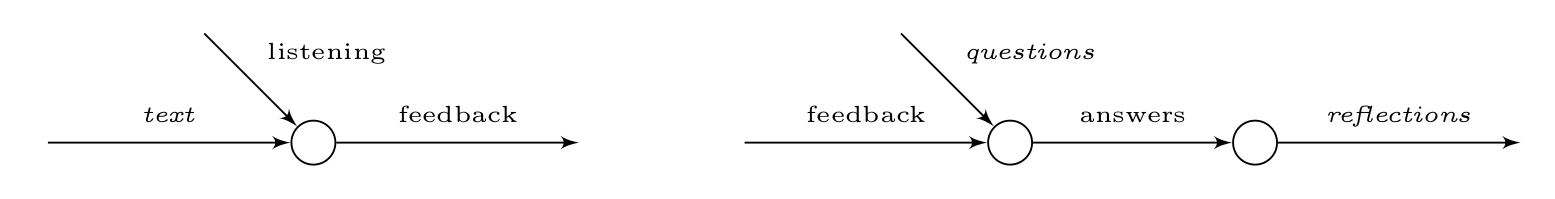
\includegraphics[width=.9\textwidth]{ww-serendipity-diagram}
%% \par}

Italicised elements (\emph{presentation}, \emph{questions}, and
\emph{reflections}) are the responsibilities of the presenting author,
and the upright elements (listening, feedback, and
answers) are the responsibilities of the attendant critics.
%
The system as a whole can be further decomposed into generative
components as follows:

\bigskip

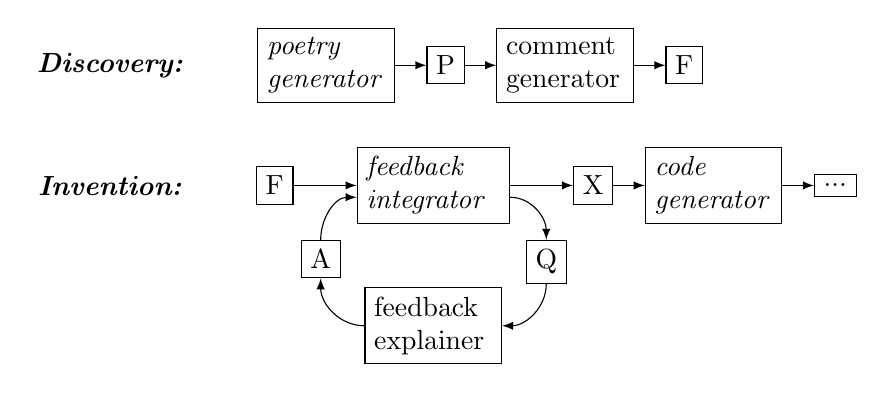
\begin{tikzpicture}[
single/.style={draw, anchor=text, rectangle},
]
\node (discovery) {\textbf{\emph{Discovery:}}};
% poet generates poem
\node[single, right=8mm of discovery.east,text width=1.5cm] (poet) {\emph{poetry generator}};
\node[single, right=4mm of poet.east] (poem) {P};
\draw [-latex] (poet.east) -- (poem.west);
% critic listens to poem and offers feedback
\node[single, right=4mm of poem.east,text width=1.5cm] (critic) {comment generator};
\draw [-latex] (poem.east) -- (critic.west);
\node[single, right=4mm of critic.east] (feedback) {F};
\draw [-latex] (critic.east) -- (feedback.west);

%%% Next phase
\node[below=1cm of discovery] (invention) {\textbf{\emph{Invention:}}};
% poet integrates feedback
\node[single, right=8mm of invention.east] (feedbackcont) {F};
\node[single, right=8mm of feedbackcont.east,text width=1.7cm] (integrator) {\emph{feedback integrator}};
\draw [-latex] (feedbackcont.east) -- (integrator.west);

\node[single, below=8mm of integrator.south,text width=1.5cm] (explainer) {feedback explainer};

\node[single, below right=2mm and 2mm of integrator] (question) {Q};
\node[single, below left=2mm and 2mm of integrator] (answer) {A};

\draw[-latex] ([yshift=-1.5mm]integrator.east) to [out=0,in=90] (question.north) ;
\draw[-latex] (question.south) to [out=270,in=0] (explainer.east) ;
\draw[-latex] (explainer.west) to [out=180,in=270] (answer.south) ;
\draw[-latex] (answer.north) to [out=90,in=180] ([yshift=-1.5mm]integrator.west) ;

\node[single, right=8mm of integrator.east] (problem) {X};

\draw [-latex] (integrator.east) -- (problem.west);

% poet reflects on feedback and updates codebase

\node[single, right=4mm of problem.east,text width=1.5cm] (pgrammer) {\emph{code}\\ \emph{generator}};

\draw [-latex] (problem.east) -- (pgrammer.west);

\node[single, right=4mm of pgrammer.east,text width=.3cm] (etc) {...};

\draw [-latex] (pgrammer.east) -- (etc.west);
\end{tikzpicture}


\bigskip

\noindent In our thought experiment, we focus on the case of hypothetical such discussions and exchange of views between computational poetry systems as our example of a situation where social circumstances could encourage serendipity. We note that similar
ideas would apply for prose and, with further adaptation, other arts.

\paragraph{Thought Experiment: Prepared mind.}
Participating systems need to be able to follow the protocol.  This
means that participating systems will need components like those
listed above. The {\tt listening} and {\tt questions} components of
the protocol correspond to $p$ and $p^{\prime}$ our model of
serendipity.  The corresponding ``comment generator'' and ``feedback
integrator'' modules in the architecture represent the primary points
of interface to the outside world.  In principle these modules need to
be prepared to deal (more or less thoughtfully) with \emph{any} text,
and in turn, with \emph{any} comment on that text.  Certain limits may
be agreed in advance; e.g.~as to genre or length in the case of texts,
and what constitutes an acceptable comment.  The ``feedback
explainer'' is closely connected with the ``comment generator'' and in
an implementation of this model they would presumably share a
codebase.  The loop for learning by asking questions as they arise is
reminiscent of the operating strategy of {\sf SHRDLU}
\cite{winograd1972understanding}.

\paragraph{Thought Experiment: Serendipity triggers.}

Although the poem is under the control of the initial generative
subsystem, it is \emph{not} under control of the listening subsystem.
The listening subsystem expects some poem, but it does not know what
poem to expect.  In this sense, the poem constitutes a serendipity
trigger $T$, not only for the listening subsystem, but for the
Workshop system as a whole.

To expand this point, note that there may be several listeners, each
sharing their own feedback and listening to the feedback presented by
others (which, again, is outside of their direct control).  This
creates further potential for serendipity, since each listener can
learn what others see in the poem.  More formally, in this case
$T^\star$ may seen as an evolving vector with shared state, but viewed
and handled from different perspectives.  With multiple agents
involved in the discussion, the ``comment generator'' module would
expand to contain its own feedback loops.

\paragraph{Thought Experiment: Bridge.}

Feedback on portions of the poem may lead the system to identify new
problems, indeed, new \emph{types} of problems that it hadn't
considered before.  The most immediately feasible case is one in which
the critic is a programmer who can directly program new concepts into
the computer \cite<cf.>{winograd1972understanding}.  However, it would
be hard to call that ``serendipity.''

We can also ask whether agents can build new concepts \emph{without}
outside intervention, starting with some basic concepts and abilities
related to poetry (e.g.~definitions of words, valence of sentiments,
metre, repetition, density, etc.) and code (e.g.~the data, functions,
and macros in which the poetic concepts and workshop protocols are
embodied).  Previous experiments with concept invention have been
fraught with questions about autonomy
\cite{ritchie1984case,lenat1984and}.  One cognitively inspired
hypothesis is that the formation of new concepts is closely related to
formation of sensory experiences \cite{milan2013kiki}.  If the
workshop participants have the capacity to identify the distinctive
features of a given poem, then training via a machine learning or
genetic algorithm approach could be used assemble a battery of
existing low-level tools that can approximate the effect.  Relatedly,
a compression process could seek to produce a given complex poetic
effect with a maximally-succinct algorithm.

The key point is that feedback on the poem -- simply describing what's
in the poem from several different points of view -- can be used to
define new problems for the system to solve.  This is not simply a
matter of decomposing the poem into pieces, but also of reconstructing
the way in which the pieces work together.  This is one of the
functions of the {\tt questions} step corresponding to $p^{\prime}$ in
our formalism: they offer the poet the opportunity to enquire about
how different pieces of feedback fit together, and learn more about
where they come from.  Although computers are currently nowhere close,
the reconstructive process may steadily approach the ideal case --
familiar to humans -- of relating to the sentiment expressed by the
poem as a whole \cite[p. 209]{bergson1983creative}.

%% Several of us are involved with a contemporary project
%% \cite{coinvent14} to develop a formal theory of concept invention,
%% focusing on \emph{concept blending}.  The additive or subtractive
%% blending of existing poetry profiles may be another way to create new
%% concepts.


%% should be possible Modifer Grammar
%% Counting Breathing Position Distribution Phonics Rhythm Repetition
%% Thematic Narrative Entropy

\paragraph{Thought Experiment: Result.} 

The final step is to take the problem or problems that were
identified, and write new code to solve them.  Several strategies for
generating a result $R$, in the form of new code, were described
above.  Now the system evaluates the new code to see whether it holds
promise.  In order to do this, it must have a way to carry out an
evaluation and judge whether $|R|>0$.  In the most straightforward
case, it would simply make changes to the draft poem that seem to
improve it in some way.  For example, the poet might remove or alter material that
elicited a negative response from a critic.  The system may proceed to
update its modules related to poetry generation.  Notably, it may also update its own
feedback modules, after reflecting on questions like: ``How might the
critic have detected that feature in my poem?''

We then develop several case studies (some historical and some imagined) showing
how serendipitous discovery+invention can work in a computational setting.
% 
\section{Discussion} \label{sec:discussion}

\subsection{Recommendations} \label{sec:recommendations}

In the diagrammatic formalism advanced in
\cite{colton-assessingprogress}, we spoke about progress with
\emph{systems} rather than with \emph{problems}.  It would be a useful
generalisation of the formalism -- and not just a simple relabelling
-- to tackle problems as well.
%
Figueiredo and Campos \cite{Figueiredo2001}, for example, describe
serendipitous ``moves'' from one problem to another.
%
However, progress with problems does not always mean transforming a
problem that cannot be solved into one that can.  Progress may also
apply to growth in the ability to posit problems.  As Deleuze writes:
``True freedom lies in the power to decide, to constitute problems
themselves'' \cite[p. 15]{deleuze1991bergsonism}.  Indeed, against any
education by means of ready-made problems, Dewey's perspective was
that
\begin{quote}
``\emph{the child's mind can be trained only in so far as the objects
    with which they are occupied arise out of their interests and
    their own problems.}''~\cite{dewey-by-mead}
\end{quote}

This was our emphasis in Section \ref{sec:unified-approach}:
developing new design patterns is closely connected with -- and in the
dynamical interpretation we prefer, effectively synonymous with --
positing new problems.  Although \cite{colton-assessingprogress}
presented a way to model creative progress at various levels of
granularity, it dealt primarily with \emph{solutions}; and although it
exhibited progress in a way that would be recognised by impartial
observers, the formalism did not focus on expositing the features that
would permit a system to actually \emph{make} creative progress.
Accordingly, we would recommend that in applying our earlier
formalism, system designers clearly record what problem a given system
solves, and the degree to which the computer was responsible for
coming up with this problem.

In \cite{stakeholder-groups-bookchapter}, we advanced a broader
programme for computational creativity, in which we argue in favour of
studying the \emph{perceptions} of creativity by various parties.  The
criteria developed in the current paper -- including the focus shift,
which we regard as fundamental -- can be used in the same way, as we
will describe below.

%% MC> Angelina is a able to read Twitter to find out what people think of
%% MC> people like Hamid Karzai, and then change the sorts of images that
%% MC> it finds as a result.  So you're going to see a happy picture of
%% MC> President Obama later next to a very angry picture of Hamid Karzai.
%% MC> While some of this might look creative and intelligent, a lot of it
%% MC> comes down to serendipity as well.  So the image you're about to see
%% MC> comes up for a Google search for terrorism that doesn't really have
%% MC> much relevance to the news article, and the sound that you're
%% MC> hearing now, the electronic drone, sounds like it's a good choice
%% MC> for a game that's about war and about feeling unsettling.  But in
%% MC> actuality I have no idea how Angelina came up with that choice.

Our proposed Writers Workshop is very different from the Turing-style
imitation game, but nevertheless may prove to be a useful aptitude
test for computer systems, and as a context in which computationally
creative programs may become aware of each other, and participate
actively in advancing the field of research.  We previously examined
perceptions of creativity in computational systems found among members
of the general public, Computational Creativity researchers, and
creative communities -- understood as human communities.  We should
now add a fourth important ``stakeholder'' group in computational
creativity research: computer systems themselves.

To make the point emphatically: the writers workshop proposed above is
very different from a traditional system ``Show and Tell'' presented
by system developers, for system developers.  Traditional academic
practices associated with presenting finished work, or even
work-in-progress, are not entirely suitable for the field of
computational creativity, where engagement between systems may exhibit
manifestly serendipitous results.  If the community does not implement
a suggestion like the one presented here, it will be missing out on a
key idea for enhancing computational creativity that has been
circulating since Turing suggested that computers should ``be able to
converse with each other to sharpen their wits''
\cite{turing-intelligent}.  Other fields, including computer Go
\cite{bouzy2001computer} and argumentation \cite{yuan2008towards} have
their own dedicated servers and protocols for exchange.  We should
move in that direction too.

There is ample room for unpredictability in such pursuits.  Creativity
may look very different to this fourth stakeholder group than it looks
to us.  In time to come, computer systems will increasingly take
leadership in matters of genre, interaction design, and their own
artistic and scientific training.  For now, our job is not at all to
get out of the way, like the parents of young adults, but rather to
participate in creating the ``play schools'' in which systems that are
quite frankly in early development can begin to socialise with each
other.
%
In \cite{stakeholder-groups-bookchapter}, we introduced nine
hypotheses related to the perception of creativity in computational
systems. 
The last of these hypotheses stated that:
\begin{quote}
``\emph{The perception of creativity in software which produces
  artefacts within a creative community will be increased if the
  software can exhibit subjective judgements about its own work and
  that of others, and defend those judgements in an accountable
  way.}''~\cite{stakeholder-groups-bookchapter}
\end{quote}
If the framework described in this paper is developed further, we may
be able to test this hypothesis in computer simulations.

Our proposed template for design patterns for participation in writers
workshops is different from, but complementary to Alexander's
framework.  Whereas Alexander focused on solutions to common
architectural problems (\emph{A place to wait}, etc.), our framework
is primarily designed to elicit and engage with new and unexpected
problems.  We presented four examples using the template, but our
intention is for the template to be used in a reflective mode by
systems to generate new patterns, in a manner appropriate to
second-order cybernetics.  Many practical issues remain to be settled
for a future computational enterprise that seeks to combine existing
design patterns and new stimuli in order to generate new, useful
design patterns.  One thing that becomes clear from this discussion is
that \emph{problem-setting} is a fundamental issue for the field of
computational creativity that will only be given due attention when
the research culture is ready to fully embrace serendipity.

\begin{quote}
``[S]\emph{ocial cybernetics must be a second-order cybernetics--a
    cybernetics of cybernetics--in order that the observer who enters
    the system shall be allowed to stipulate his own purpose: he is
    autonomous.}'' \cite[p. 286]{von2003essays}
\end{quote}

\subsection{Future Work} \label{sec:futurework}

From this, we extract recommendations for practitioners in computational creativity, and outline our own plan of work.
% \section{Conclusion} \label{sec:conclusion}

%
We began by surveying ``serendipity'', developing a broad historical
view, and describing several criteria for serendipity which we propose
to be computationally salient.  We reviewed related work; like
\citeA{andre2009discovery}, we propose a two-part definition of
serendipity: \emph{discovery} followed by \emph{invention}.
%
Adapting the ``Standardised Procedure for Evaluating Creative
Systems'' (SPECS) model from \citeA{jordanous:12}, we developed a set
of evaluation standards for serendipity.
%
We used this model to analyse prior examples of serendipity in the
context of evolutionary music improvisation and recommender systems,
and developed a thought experiment that seems able to support ``high
serendipity'' with a novel design for a computational poetry workshop.
%
We then reflected back over our definition, outlining a programme for
serendipitous computing in the pursuit of \emph{autonomy},
\emph{learning}, \emph{sociality}, and \emph{embedded evaluation}.  We
posit the following challenges, which connect with ongoing discussions
in the field:
%
\begin{itemize}
\item \emph{A primary challenge to the serendipitous operation of
  computers is developing computational agents that specify their own
  problems.}
\item \emph{A second challenge is for computational agents to learn
  more and more about the world we live in.}
\item \emph{A third challenge is for computational agents to interact
  in a recognisably social way with us and with each other, resulting
  in emergent effects.}
\item \emph{A fourth challenge is for computational agents to evaluate
  their own creative process and products.}
\end{itemize}
%
In the current work, we have limited ourselves to clarifying
conceptual issues surrounding our definition of serendipty, and
examining their design implications.
% 
We indicate several possible further directions for implementation
work in each of our case studies.  We have also drawn attention to
theoretical questions related to doing program design in an autonomous
programming context.  Our examples show that serendipity is not
foreign to computing practice.  There are further gains to be had for
research in computing by planning -- and programming -- for
serendipity.
%


\\[.5cm]
%
%% \keywords{serendipity,
%% design patterns,
%% intelligent machinery,
%% Writers Workshops}
\end{abstract}


\tableofcontents

\section{Introduction}

Although computational creativity is well studied in both theory and
practice, the role of \emph{serendipity} has often not been discussed
in this field -- even though serendipity has played a well-documented
role in historical instances of scientific and technical creativity.
One reason for this omission may be that the field of computational
creativity has tended to focus on artistic creativity.  But
serendipity is increasingly seen as relevant within the arts
\cite{mckay-serendipity} and other creative enterprises
\cite{kakko2009homo,engineering-serendipity}: it is managed and
encouraged with methods ranging from architecture to data science.
%
An interdisciplinary perspective on the phenomenon of serendipity
promises further illumination.  Here, we consider the potential for
formalising this concept and investigate its utility as a new
framework for computational creativity.

Serendipity centres on reassessment.  For example, a non-sticky
``superglue'' that no one was quite sure how to use turned out to be
just the right ingredient for 3M's Post-it\texttrademark\ notes.
%
Serendipity is related, firstly, to deviations from expected or
familiar patterns, and secondly, to new insight.
%
When we consider the practical uses for weak glue, the possibility
that a life-saving antibiotic might be found growing on contaminated
petri dishes, and or the idea that cockle-burs could be anything but
annoying, we encounter radical changes in the evaluation of what's
interesting.  In the \emph{d\'enouement}, what was initially
unexpected is found to be both explicable and useful.

Van Andel \citeyear{van1994anatomy} -- echoing Poincar\'e's
\citeyear{poincare1910creation} (negative) reflections on the potential
for a purely computational approach to mathematics -- claimed that:
\begin{quote}
``\emph{Like all intuitive operating, pure serendipity is not amenable
    to generation by a computer.  The very moment I can plan or
    programme `serendipity' it cannot be called serendipity
    anymore}.'' \cite{van1994anatomy}
\end{quote}
We believe that serendipity is not so mystical as such statements
might seem to imply, and in Section \ref{sec:discussion} we indicate
van Andel's ``patterns of serendipity'' are likely to be highly
applicable in computational settings.

First, in
Section \ref{sec:literature-review}, we survey the broad literature on
serendipity. Then in Section \ref{sec:background} we present our formal
definition of serendipity, and examine related work that has applied
the concept of serendipity in a computational context. Section \ref{sec:connections-to-formal-definition} makes connections from historical examples of
serendipitous discovery and invention to our formal model.  Section
\ref{sec:computational-serendipity} then presents case studies and
thought experiments in terms of this model.  Section
\ref{sec:discussion} offers recommendations for researchers working in
computational creativity (a key research area concerned with the computational modelling of serendipity), and describes our own plans for future
work.  Section \ref{sec:conclusion} reviews the argument and
summarises the limitations of our analysis.



\section{Literature review} \label{sec:literature-review}

In this section, we give a short overview covering the etymology of
the term ``serendipity'' and trace its development in order to pin
down the key commonalities from many definitions and instances.  In
particular, we point out key conditions of serendipity, their
components and general characteristics, including environmental
factors.  The structure of this section follows and updates an earlier
survey from \citeA{pease2013discussion}, drawing connections with our
formal model described above.

\subsection{Etymology and selected definitions} \label{sec:overview-serendipity}
The English term ``serendipity'' derives from the 1302 long poem \emph{Eight Paradises}, written in Persian by the Sufi poet Am\={\i}r Khusrow in Uttar Pradesh.\footnote{\url{http://en.wikipedia.org/wiki/Hasht-Bihisht}}  In the English-speaking world, its first chapter became known as ``The Three Princes of Serendip'', where ``Serendip'' represents the Old Tamil-Malayalam word for Sri Lanka (%{\tam சேரன்தீவு},
\emph{Cerantivu}), ``island of the Ceran kings.''

The term ``serendipity'' is first found in a 1757 letter by Horace Walpole to Horace Mann:
\begin{quote}
\emph{``This discovery is almost of that kind which I call serendipity, a very expressive
word} \ldots \emph{You will understand it better by the derivation than by the
definition. I once read a silly fairy tale, called The Three Princes of Serendip:
as their Highness travelled, they were always making discoveries, by accidents
\& sagacity, of things which they were not in quest of}[.]''~\cite[p. 633]{van1994anatomy}
\end{quote}
The term became more widely known in the 1940s through studies of serendipity as a factor in scientific discovery, surveyed by Robert Merton and Elinor Barben \citeyear{merton} in their 1957 analyis ``The Travels and Adventures of Serendipity, A Study in Historical Semantics and the Sociology of Sciences''.  Merton and Barben define the term as follows:
\begin{quote}
\emph{``The serendipity pattern refers to the fairly common experience of observing
an unanticipated, anomalous and strategic datum which becomes the occasion
for developing a new theory or for extending an existing theory.''} \cite[p. 635]{van1994anatomy}
\end{quote}
In 1986, Philippe Qu\'eau described serendipity as ``the art of
finding what we are not looking for by looking for what we are not
finding'' \cite{eloge-de-la-simulation}, as quoted in
\cite[p. 121]{Campos2002}.  Pek van Andel
\citeyear[p. 631]{van1994anatomy} describes it simply as ``the art of
making an unsought finding''.


Roberts \citeyear[pp. 246--249]{roberts} records 30 entries for the term ``serendipity'' from English language dictionaries dating from 1909 to 1989.  
%
Classic definitions require the investigator not to be aware of the problem they serendipitously solve, but this criterion has largely dropped from dictionary definitions. Only 5 of Roberts' collected definitions explicitly say ``not sought for.''  Roberts characterises ``sought findings'' in which an accident leads to a discovery with the term \emph{pseudoserendipity} \cite{chumaceiro1995serendipity}.
%
While Walpole initially described serendipity as an event, it has
since been reconceptualised as a psychological attribute, a matter of
sagacity on the part of the discoverer: a ``gift'' or ``faculty'' more
than a ``state of mind.''  Only one of the collected definitions, from
1952, defined it solely as an event, while five define it as both
event and attribute.

However, there are numerous examples that exhibit features of
serendipity which develop on a social scale rather than an individual
scale.  For instance, between Spencer Silver's creation of high-tack,
low-adhesion glue in 1968, the invention of a sticky bookmark in 1973,
and the eventual launch of the distinctive canary yellow re-stickable
notes in 1980, there were many opportunities for
Post-its\texttrademark\ \emph{not} to have come to be
\cite{tce-postits}. Accordingly, Merton and Barber argue that the
psychological perspective needs to be integrated with a
\emph{sociological} one.\footnote{ ``For if chance favours prepared
  minds, it particularly favours those at work in microenvironments
  that make for unanticipated sociocognitive interactions between
  those prepared minds. These may be described as serendipitous
  sociocognitive microenvironments'' \cite[p. 259--260]{merton}.}
Large-scale scientific and technical projects generally rely on the
``convergence of interests of several key actors''
\cite{companions-in-geography}, along with other supporting cultural
factors.  Umberto Eco \citeyear{eco2013serendipities} focuses on the
historical role of serendipitous mistakes and falsehoods in the
production of knowledge.

It is important to note that serendipity is usually discussed within
the context of \emph{discovery}, rather than \emph{creativity},
although in typical parlance these terms are closely related
\cite{jordanous12jims}.  In our definition of serendipity, we have
made use of Henri Bergson's distinction:
\begin{quote}
``\emph{Discovery, or uncovering, has to do with what already exists,
    actually or virtually; it was therefore certain to happen sooner
    or later.  Invention gives being to what did not exist; it might
    never have happened.}''~\cite{bergson2010creative}
\end{quote}
As we have indicated serendipity would seem to require features of
both; that is, the discovery of something unexpected and the invention
of an application for the same.  We must complement \emph{analysis}
with \emph{synthesis} \cite{delanda1993virtual}.  The balance between
these two features will differ from case to case.

In the next subsection we will review several historical examples.
First, one further point should be made with reference to the ``The
Three Princes of Serendip''.  Prior to Walpole's coinage, this story
had been adapted by Voltaire into an early chapter of \emph{Zadig},
and in turn ``the method of Zadig'' informed subsequent approaches
both to fiction writing and natural science.  This method is rooted
firstly in discovery:

\begin{quote}
``[Zadig] \emph{pry’d into the Nature and Properties of Animals and
    Plants, and soon, by his strict and repeated Enquiries, he was
    capable of discerning a Thousand Variations in visible Objects,
    that others, less curious, imagin’d were all
    alike.}''~\cite[pp. 21--22]{zadig}
\end{quote}

\noindent Secondly, from disparate observations, Zadig is often able
to assemble a coherent picture:
\begin{quote}
\emph{It was his peculiar Talent to render Truth as obvious as
  possible: Whereas most Men study to render it intricate and
  obscure.}~\cite[p. 54]{zadig}
\end{quote}
Similarly, but in reverse, a coherent picture may be reduced to
fragmented pieces each of which may tell a very different story from
the whole.  This is illustrated in Zadig's misadventure with a broken
tablet, in which one fragment of a poem of praise reads as treasonous
provocation.  In describing the various features of serendipity below,
we will draw connections with the schematic diagram presented in
Section \ref{specs-overview}, in order to unfold the multifaceted
notion of serendipity.

\subsection{Connections between prior literature on serendipity and our formal definition} \label{sec:connections-to-formal-definition}

\subsubsection*{Key condition for serendipity}

\begin{itemize}
\item \textbf{Focus shift}: ``\emph{After removing several of the
  burdock burrs (seeds) that kept sticking to his clothes and his
  dog's fur,}~[de Mestral]~\emph{became curious as to how it
  worked. He examined them under a microscope, and noted hundreds of
  `hooks' that caught on anything with a loop, such as clothing,
  animal fur, or hair. He saw the possibility of binding two materials
  reversibly in a simple fashion, if he could figure out how to
  duplicate the hooks and loops.}''~\cite{wiki:velcro}
%
\inlineitem{This corresponds to the identification of $T^\star$, which
  is common to both sides of the diagram.  \citeA{creativity-crisis}
  write that: ``To be creative requires divergent thinking (generating
  many unique ideas) and then convergent thinking (combining those
  ideas into the best result).''  Accordingly $T^\star$ may be thought
  of as an evolving vector of interesting possibilities or ``strategic data'' \cite[p. 507]{merton1948bearing}.  In de
  Mestral's case, the initial idea of a hook-and-loop fastener
  occurred in 1941 -- followed by a full decade of experimentation
  before he was ready to file a patent claim.  }
\end{itemize}

\subsubsection*{Components of serendipity}

\begin{itemize}
\item \textbf{Prepared mind}: 
Fleming's ``prepared mind'' included his focus
on carrying out experiments to investigate influenza as well as his
previous experience that foreign substances in petri dishes can kill
bacteria.  He was concerned above all with the question ``Is there a
substance which is harmful to harmful bacteria but harmless to human
tissue?''  \cite[p. 161]{roberts}.
%%
%
\inlineitem{This corresponds to the prior
  training $p$ and $p^{\prime}$ in our diagram.}
\item \textbf{Serendipity trigger}: The trigger does not directly
  cause the outcome, but rather, inspires a new insight.  It was long
  known by Quechua medics that cinchona bark stops shivering.  In
  particular, it worked well to stop shivering in malaria patients, as
  was observed when malarial Europeans first arrived in Peru.  The
  joint appearance of shivering Europeans and a South American remedy
  was the trigger.  That an extract from cinchona bark can cure and
  can even prevent malaria was subsequently revealed.
%
\inlineitem{This corresponds to the stimulus $T$ in our diagram.}
%%
\item \textbf{Bridge}: These include reasoning techniques, such as
  abductive inference (what might cause a clear patch in a petri
  dish?); analogical reasoning (de Mestral constructed a target domain
  from the source domain of burs hooked onto fabric); and conceptual
  blending (Kekul\'e blended his knowledge of molecule structure with
  his vision of a snake biting its tail).  The bridge may also rely on
  new social arrangements, such as the formation of cross-cultural
  research networks.
%
\inlineitem{This corresponds to the actions based on $p^{\prime}$
  taken on $T^\star$ leading to $R$.}
%%
\item \textbf{Result}: This may be a new product, artefact, process,
  hypothesis, a new use for a material substance, and so on.  The
  outcome may contribute evidence in support of a known hypothesis, or
  a solution to a known problem.  Alternatively, the result may itself
  be a {\em new} hypothesis or problem.  The result may be a
  ``pseudoserendipitous'' in the sense that it was {\em sought}, while
  nevertheless arising from an unknown, unlikely, coincidental or
  unexpected source.  More classically, it is an \emph{unsought}
  finding, such as the discovery of the Rosetta stone.
%
\inlineitem{This corresponds to our $R$.  Note that $R$ may imply
  updates to $p$ or $p^{\prime}$ in further phases of research.}
\end{itemize}

\subsubsection*{Dimensions of serendipity}

Whereas the foregoing items are the central features of the
definition, the following further characterise the circumstances under
which serendipity occurs in practice.

\begin{itemize}
\item \textbf{Chance}: Fleming \citeyear{fleming} noted: ``There are
  thousands of different moulds'' -- and ``that chance put the mould
  in the right spot at the right time was like winning the Irish
  sweep.''
%
\inlineitem{One must assume that relatively few triggers $T^\star$
  that are identified as interesting actually lead to useful results;
  in other words, the process is fallible.}
%%
\item \textbf{Curiosity}: Venkatesh Rao \citeyear{rao2011tempo} refers
  to a \emph{cheap trick} that takes place early on in a narrative in
  order to establish the preliminary conditions of order.  Curiosity
  with can play this role, and can dispose a creative person to begin,
  or to continue, a search into unfamiliar territory.
%
\inlineitem{The prior training $p$ causes interesting features to be
  extracted, even if they are not necessarily useful; $p^{\prime}$
  asks how these features \emph{might} be useful.  }
%%
\item \textbf{Sagacity}: This old-fashioned word is related to
  ``wisdom,'' ``insight,'' and especially to ``taste'' -- and
  describes the attributes, or skill, of the discoverer that
  contribute to forming the bridge between the trigger and the result.
  In many cases, such as an entanglement with cockle-burs, many others
  will have already been in a similar position and not obtained an
  interesting result.  Once a phenomenon has been identified as
  interesting, the disposition of the investigator may lead to a
  dogged pursuit of a useful application or improvement.
%
\inlineitem{Rather than a simple look-up
  rule, $p^{\prime}$ involves creating new knowledge.}
%%
\item \textbf{Value}: Note that the chance ``discovery'' of, say, a
  \pounds 10 note may be seen as happy by the person who finds it,
  whereas the loss of the same note would generally be regarded as
  unhappy.  Positive judgements of serendipity by a third party would
  be less likely in scenarios in which ``One man's loss is another
  man's gain'' than in scenarios where ``One man's trash is another
  man's treasure.''  If possible we prefer this sort of independent
  judgement \cite{jordanous:12}.
%
\inlineitem{The evaluation $|R|>0$ may be carried out ``locally'' (as
  an embedded part of the process of invention of $R$) or ``globally''
  (i.e.~as an external process).  }
\end{itemize}

\subsubsection*{Environmental factors}

\begin{itemize}
\item \textbf{Dynamic world}: Information about the world develops
  over time, and is not presented as a complete, consistent whole.  In
  particular, value may come later.  Van Andel
  \citeyear[p. 643]{van1994anatomy} estimates that in twenty percent
  of innovations ``something was discovered before there was a demand
  for it.''
%
\inlineitem{$T$ (and $T^\star$) appears within a stream of data with
  indeterminacy.  There is a further feedback loop, insofar as
  products $R$ influence the future state.}
%%
\item \textbf{Multiple contexts}: One of the dynamical aspects at play
  may be the discoverer going back and forth between different
  contexts, with different stimuli.  3M employee Arthur Fry sang in a
  church choir and needed a good way to mark pages in his hymn book;
  he happened to have been attending seminars offered by his colleague
  Silver about restickable glue.
%
\inlineitem{This is reflected directly in our model by the difference
  between the ``context of discovery'' involving prior preparations
  $p$, and the ``context of invention'' involving prior preparations
  $p^{\prime}$.  Both of these may be subdivided further.}
%%
\item \textbf{Multiple tasks}: Even within what would typically be
  seen as a single context, a discoverer may take on multiple tasks
  that segment the context into sub-contexts, or that cause the
  investigator to look in more than one direction.  The tasks may have
  an interesting \emph{overlap}, or they may point to a \emph{gap} in
  knowledge.  As an example of the latter, Penzias and Wilson used a
  large antenna to detect radio waves that were relayed by bouncing
  off of satellites.  After they had removed interference effects due
  to radar, radio, and heat, they found residual ambient noise that
  couldn't be eliminated \cite{wiki:cosmic-radiation}.
%
\inlineitem{Both $T$ and $T^\star$ may be multiple, causing an
  individual process to fork into communicating sub-processes that
  involve different skills sets.}
%%
\item \textbf{Multiple influences}: The ``bridge'' from trigger to
  result is often found through a social network, thus, for instance
  Penzias and Wilson only understood the significance of their work
  after reading a preprint by Jim Peebles that hypothesised the
  possibility of measuring radiation released by the big bang
  \cite{wiki:cosmic-radiation}.
%
\inlineitem{The process as a whole may be multiplied out among
  different communicating investigators.}
\end{itemize}

% \section{Foundational work} \label{sec:foundations}

%% \begin{figure}
%% \centering
%% \includegraphics[width=.85\textwidth]{poetic-couplets}
%% \caption{A simple flow chart defined in the {\sf FloWr} system \label{fig:simple-flow-chart}}
%% \end{figure}

% AJ *** How is this content relevant? Seems like quite a jump from the last section. I've added a sentence to start the paragraph off ***
In moving towards computational models of serendipity, we are
supported by prior foundational work providing a theoretical framework
and a virtual environment for exploring computational creativity.  In
\citeA{colton-assessingprogress}, we introduced a diagrammatic
formalism for keeping track of progress made in creative computational
systems. An example, pictured in Figure \ref{fig:poetry-progress},
shows how the second iteration of a poetry system gains the ability to
automatically apply aesthetic judgements in order to select a
preferred poem from a larger set of generated examples, once the
programmer has translated (by hand) the relevant aesthetic measures.
\begin{wrapfigure}{l}{4.1cm}
\centering
%\vspace{-30pt}
\resizebox{.23\textwidth}{!}{%
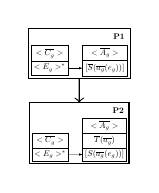
\begin{tikzpicture}[
single/.style={draw, anchor=text, rectangle},
double/.style={draw, anchor=text, rectangle split,rectangle split parts=2},
triple/.style={draw, anchor=text, rectangle split,rectangle split parts=3},
quadruple/.style={draw, anchor=text, rectangle split,rectangle split parts=4}
]
%% beginning of FIRST box
\node[single,scale=0.3] (first) at (0, 0) {
  \tikz{
%\draw[step=1cm,gray,very thin] (-4,-4) grid (4,4);
\node[double] (firstA) at (-2,0) {$<\overline{C_g}>$
  \nodepart{second}{$<E_g>^{*}$}
};
\node[double,right=6mm of firstA.east] (firstB) {$<\overline{A_g}>$
  \nodepart{second}{$[\overline{S}(\overline{a_g}(e_g))]$}
};
\draw [-latex] (firstA.two east) -- (firstB.two west);
\node[above = .01cm of firstB,label={[label distance=2mm]10:{\textbf{P1}}},inner sep=1pt]{};
}
};
%% end of first box

%% beginning of SECOND box
\node[single,scale=0.3,below=3mm of first, inner sep=1mm] (second) {
  \tikz{
%\draw[step=1cm,gray,very thin] (-4,-4) grid (4,4);
\node[double] (firstA) at (-2,0) {$<\overline{C_g}>$
  \nodepart{second}{$<E_g>^{*}$}
};
\node[triple,right=6mm of firstA.one east,yshift=.3mm] (firstB) {$<\overline{A_g}>$
  \nodepart{second}{$\overline{T}(\overline{a_g})$}
  \nodepart{third}{$[S(\overline{a_g}(e_g))]$}
};
\draw [-latex] (firstA.two east) -- (firstB.three west);
\node[above = .01cm of firstB,label={[label distance=2mm]10:{\textbf{P2}}},inner sep=1pt]{};
}
};;
%% end of second box

\draw[->] (first) -- (second);
\end{tikzpicture}}
\vspace{-5pt}
\caption{Progress in developing a poetry system\label{fig:poetry-progress}}
\vspace{-20pt}

\end{wrapfigure}
Progress amounts to more sophisticated processing, and, in the
notation, frequently corresponds to the removal of ``bars'' --
indicating that the system can do something that was formerly done by
a programmer.
%
Thus, this formalism keeps track both of the overall structure of
computational systems, and which actors that are responsible for which
actions within a given instance of the system.
%
As we develop models and systems that people would describe as
serendipitous with reference to the criteria listed in Section
\ref{sec:characteristics}, there will be more to account for.  

\smallskip

For example, we will need to model dynamically changing environments
and a computational version of a prepared mind.
%
To explore these features, are working with a system called {\sf
  FloWr}, portrayed with a screenshot in Figure \ref{fig:being-blunt}.
In {\sf FloWr}, users can construct complex flowcharts composed of
individual ProcessNodes, through which information flows and is
transformed.  The figure depicts a flowchart that has constructed a
poem based on live output from Twitter for the query ``blunt''.  The
dynamic aspects of this environment are threefold: (\emph{i}) some of
the nodes in the flowcharts access online news and social media sites,
which change rapidly from minute to minute; (\emph{ii}) the software
itself can construct new flowcharts, as described in
\cite{charnley2014flowr}; and (\emph{iii}) we are building a community
of ProcessNode builders around the online version of {\sf FloWr},
newly developed since the publication of \cite{charnley2014flowr} in
order to facilitate the direct involvement of other Computational
Creativity researchers.

\begin{figure}
\centering
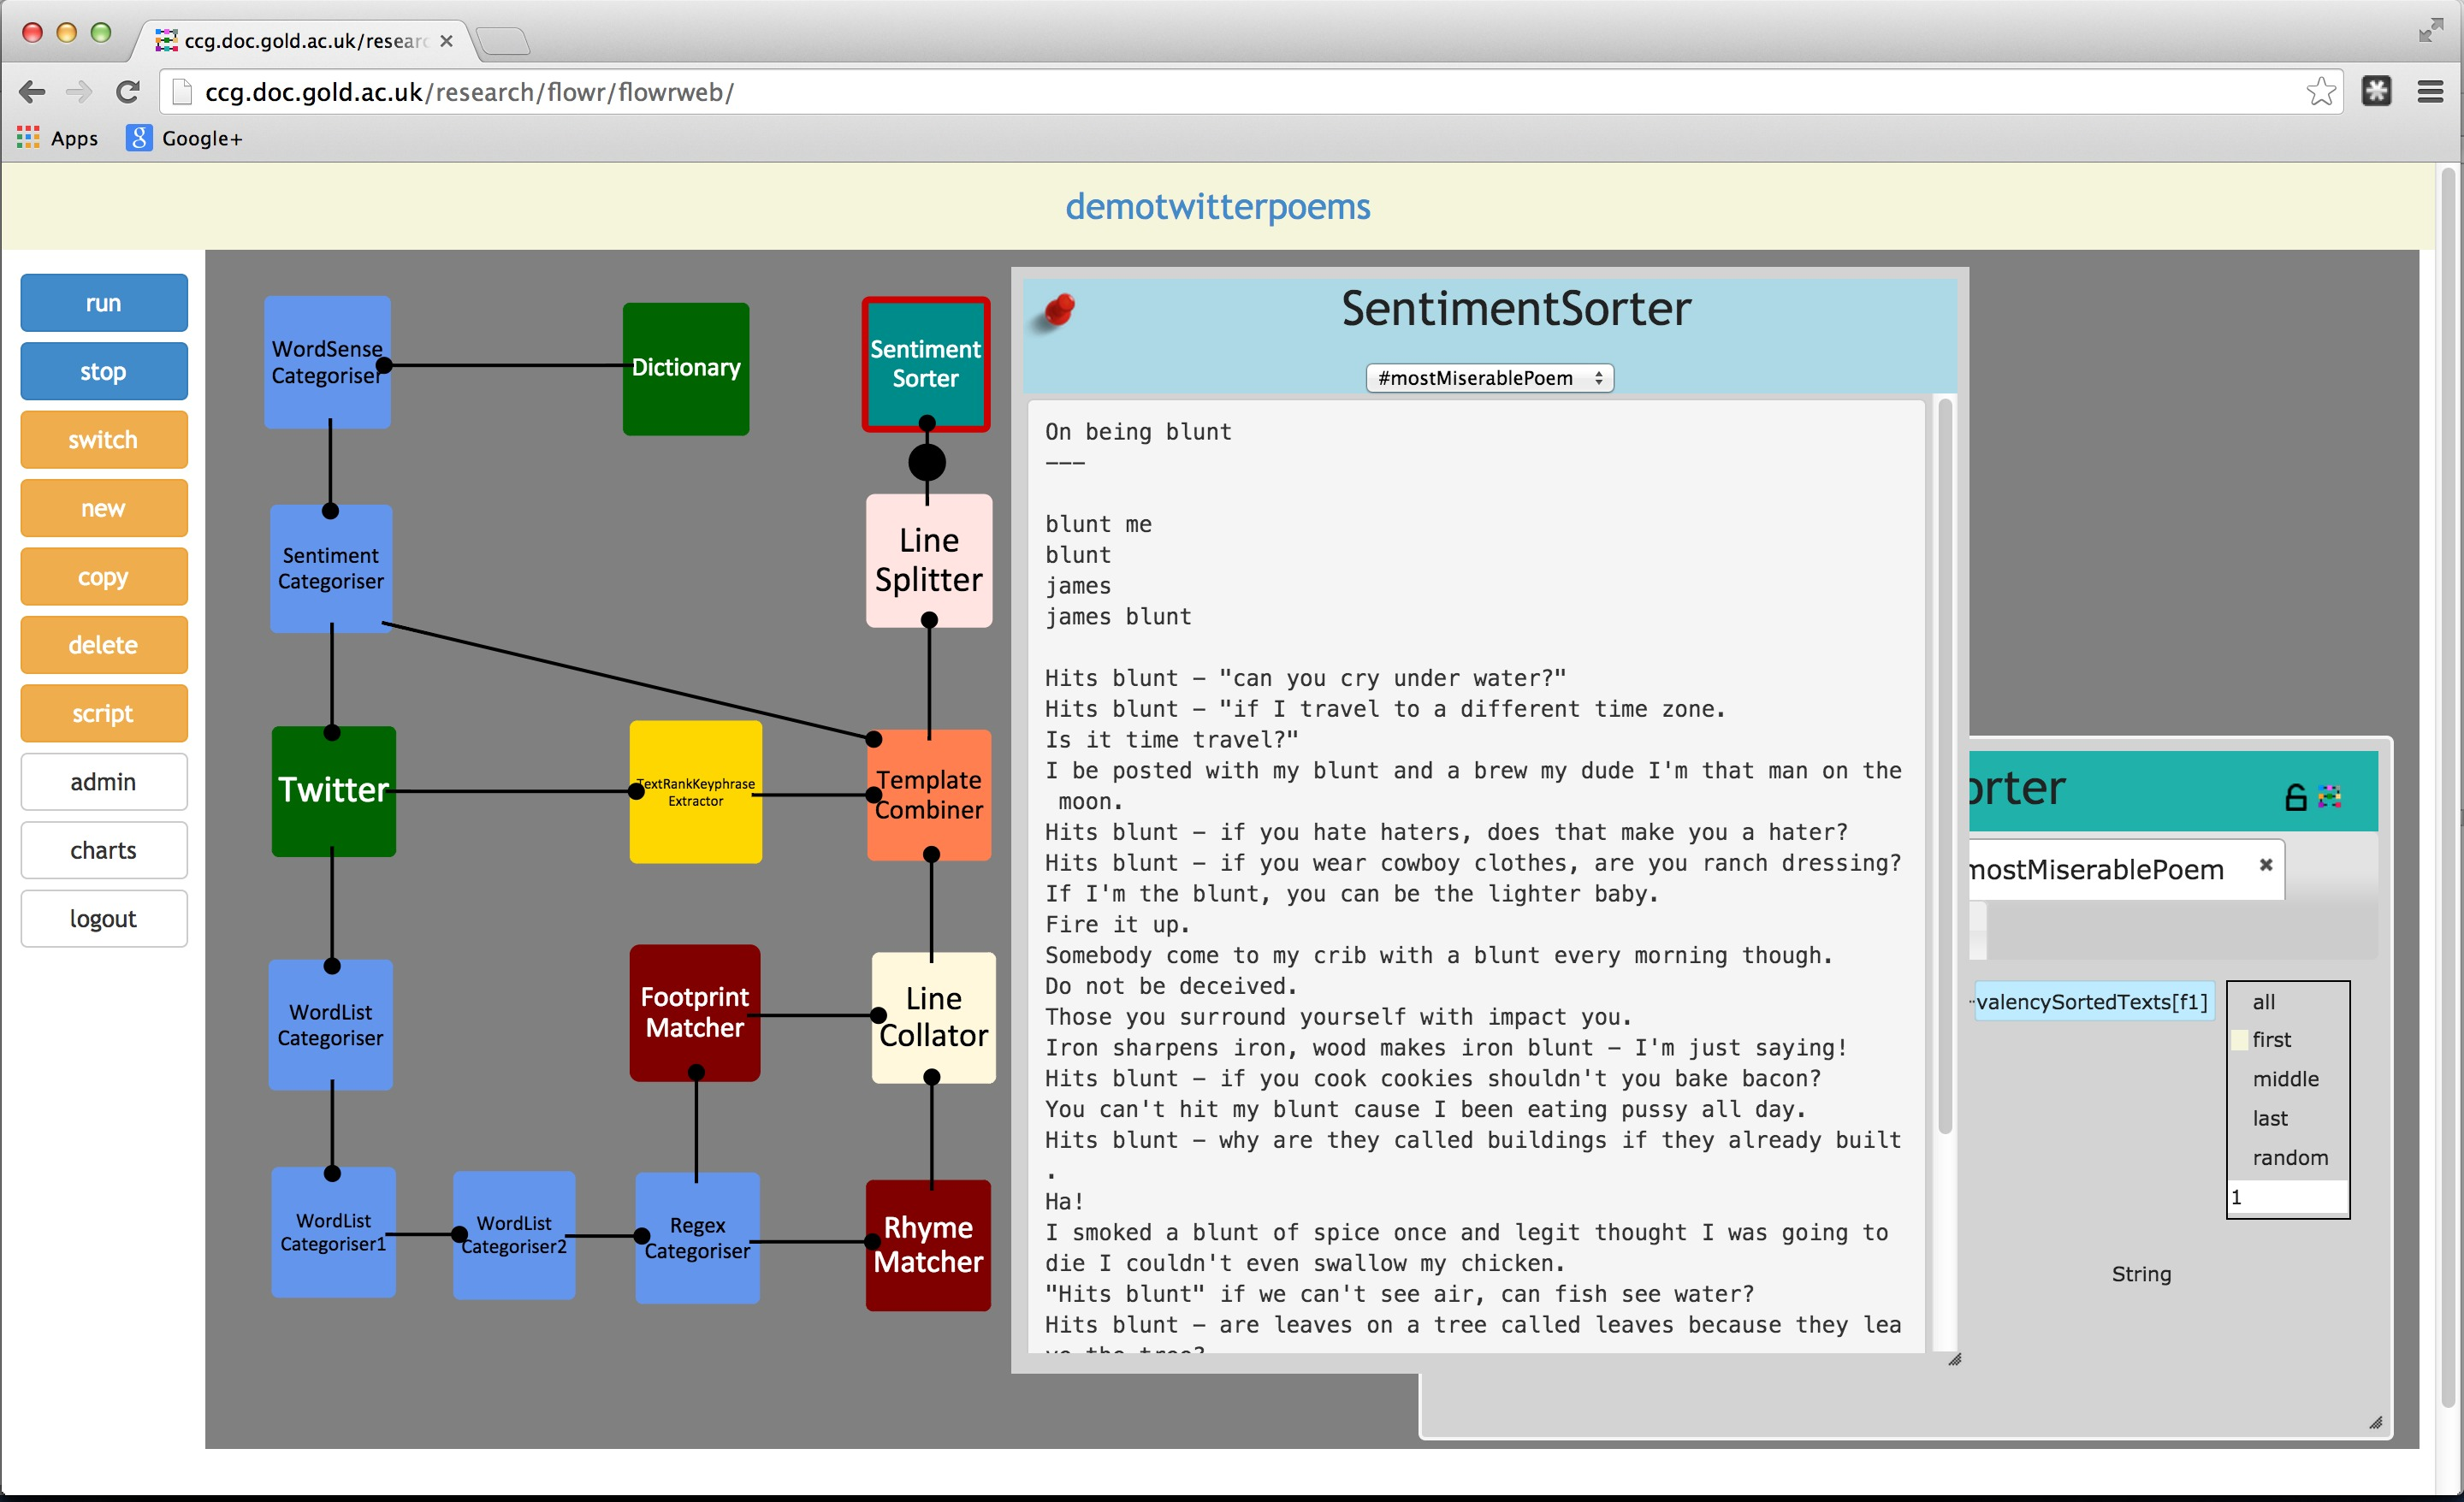
\includegraphics[width=.95\textwidth]{being-blunt}
\caption{A sample poem generated by {\sf FloWr}\label{fig:being-blunt}}
\end{figure}


When {\sf FloWr} constructs flowcharts for itself, while each is
semantically plausible (i.e., they pass the right type of data from
ProcessNode to ProcessNode), many fail -- for instance, because the
available data is limited, or is narrowed down too quickly.  In fact,
the best results in \cite{charnley2014flowr} were at 20\%, i.e., 80\%
of the flowcharts that were constructed failed to produce output.
Each of these failures can be saved as an outstanding problem in {\sf
  FloWr}'s prepared mind.  As data changes and as new nodes are
written and uploaded to the system, {\sf FloWr} will be able to replace nodes,
update data sources, and in general rearrange flowcharts in order to
see if it can fix a broken flowchart.

For instance, suppose a ProcessNode developer wrote and uploaded a
node to mine data from a new social network, in order, say, to produce
textual summaries of world events.  {\sf FloWr} may take that node
and substitute it in the place of an old ``FaceBook'' node in a broken
poetry flowchart. If the replacement worked, and output was produced,
this could be seen as a serendipitous occurrence: {\sf FloWr} will
have taken advantage of the dynamically changing environment -- in
which new social networks come and go, and in which text summaries may
work better in some cases than in others -- to resolve an outstanding
problem in text generation.

The next stage for the {\sf FloWr} system will be to modify it along
these lines, to make it able to adapt to the dynamically changing
environment, and to perform experiments where we monitor potentially
serendipitous scenarios. Such experiments will be similar to those we
tried with the HR2 system in \cite{pease2013discussion}, but improved
because in this earlier effort, we had to break working processes in
order to serendipitously fix them.  The new experiments, the scenarios
will be more realistic, i.e., there will be a catalogue of genuine
open problems waiting to be solved.  Understanding how to work with
this catalogue and the associated experimental process will, of
course, be used to further the computational model of serendipity.  We
discuss one direction for such experiments in Section
\ref{sec:writers-workshop}.

\section{Serendipity in a computational context} \label{sec:computational-serendipity}

The 13 criteria from Section \ref{sec:literature-review}
specify the conditions and preconditions that are conducive to
serendipitous discovery.  Here, we revisit each of these criteria and
briefly summarise how they can be thought about from a computational
point of view.
% What is the goal of the computation (input and output)
% Why is it appropriate (formal spec e.g. considering externalities)
% what is the logic of the strategy by which it can be carried out.

\textbf{[Do we need to include the partial repetition below or is the
    above formal enough?  Could these bulleted ideas be condensed into
    one or two paragraphs]}

\subsubsection*{Key condition for serendipity}

\begin{itemize}
\item \textbf{Focus shift}: A focus shift is linked to re-evaluation
  of data, processes, or products.  It may precipitate changes in the
  entire framework of evaluation or its effects may be more contained.
  Such reevaluation could be modelled using a multi-agent
  architecture, in which each agent has a goal and evaluates generated
  products relative this goal, but in which agents also share their
  products with other, who then evaluate them against their own
  metrics.
\end{itemize}

\subsubsection*{Components of serendipity}

\begin{itemize}
\item \textbf{Prepared mind}: This comprises the background knowledge,
  unsolved problems, current goal, programming, and operating
  environment of a computational system.
%%
\item \textbf{Serendipity trigger}: The generation or observation of a
  potentially novel example, concept, or conjecture, etc., which
  precedes a discovery in a computational system.\footnote{Triggers
    are often examples without an explanation, rather than
    wholly-formed concepts.}  The trigger is outside of the direct
  control of the system components responsible for evaluations.
%%
\item \textbf{Bridge}: Reasoning and/or programmatic interaction
  brings about a focus shift at an opportune juncture, building on
  prior preparation and on the serendipity trigger.  The bridge may be
  constructed on the basis of logical methods, analogies, conceptual
  blending, evolutionary search, automated theory formation and may
  draw on interactions with other systems.
%%
\item \textbf{Result}: The discovery itself may be a new product,
  artefact, process, hypothesis, use for an object, etc., generated by
  computational means, which may influence the future operations of
  the system.
\end{itemize}

\subsubsection*{Dimensions of serendipity}

\begin{itemize}
\item \textbf{Chance}: Controlled randomness in AI systems is
  well-established, e.g. in Genetic Algorithms and search.  Chance
  also applies in connection with an under-determined outside world
  (see below).
%%
\item \textbf{Curiosity}: The system needs to expend discretionary
  computational effort on the serendipity trigger.  This may be
  accompanied by system features that an observer would describe as
  playfulness, inventiveness, and the drive to experiment or
  understand.
%%
\item \textbf{Sagacity}: Sagacity be modelled by employing reasoning
  over multiple application domains simultaneously; or, again, with a
  social analogue in cases where the system does not know, but ``knows
  who to ask.''
%%
\item \textbf{Value}: The result should be interesting or useful, as
  judged by the system, the programmer, the user, or another party
  (potentially another system).
\end{itemize}

\subsubsection*{Environmental factors}

\begin{itemize}
\item \textbf{Dynamic world}: Connections with other systems, data
  sources, or user input, e.g., via the web, which is highly dynamic --
  or in the context of a larger simulation.
%%
\item \textbf{Multiple contexts}: Reasoning which operates across
  domains, such as analogical reasoning, or that considers multiple
  perspectives, as in systems with social awareness.
%%
\item \textbf{Multiple tasks}: Multiple goals or targets that compete
  for resources.  The system may be implemented using a multithreaded,
  parallel processing design.
%%
\item \textbf{Multiple influences}: This may again be modelled as a
  multi-agent systems, as or multiple interacting systems, each with
  different knowledge and goals.  The source of unexpectedness may be
  arise on various levels, and a system may bring this to bear using
  techniques of reflection.
\end{itemize}

% \subsection{Proposed experiment: A Writers Workshop for Systems} \label{sec:writers-workshop}

Richard Gabriel \cite{gabriel2002writer} describes the practise of
Writers Workshops that has been put to use for over a decade within
the Pattern Languages of Programming (PLoP) community.  The basic
style of collaboration originated much earlier with groups of literary
authors who engage in peer-group critique.  Some literary workshops
are open as to genre, and happy to accommodate beginners, like the
Minneapolis Writers
Workshop\footnote{\url{http://mnwriters.org/how-the-game-works/}};
others are focused on professionals working within a specific genre,
like the Milford Writers
Workshop\footnote{\url{http://www.milfordsf.co.uk/about.htm}}.  The
practices that Gabriel describes are fairly typical.  Authors come
with work ready to present, and read a short sample, which is then
discussed and constructively critiqued by attendees.  Presenting
authors are not permitted to rebut these comments.  The commentators
generally summarise the work and say what they have gotten out of it,
discuss what worked well in the piece, and talk about how it could be
improved.  The author listens and may take notes; at the end, he or
she can then ask questions for clarification.  Generally, non-authors
are either not permitted to attend, or are asked to stay silent
through the workshop, and perhaps sit separately from the
participating authors/reviewers.  There are similarities between the
Writers Workshops and classical practices of group composition
\cite{jin1975art} and dialectic \cite{dialectique}, and the workshop
may be considered an artistic or creative space in its own right.

In PLoP workshops, authors present design patterns and pattern
languages, or papers about patterns, rather than more traditional
literary forms like poems, stories, or chapters from novels.  Papers
must be workshopped at a PLoP or EuroPLoP conference in order to be
considered for the \emph{Transactions on Pattern Languages of
  Programming} journal.  A discussion of writers workshops
in the language of design patterns is presented by
Coplien and Woolf \cite{coplien1997pattern}.  Their patterns include:
\begin{center}
{\small
\begin{tabular}{l@{\hspace{.2cm}}l@{\hspace{.2cm}}l}
\emph{Open Review} & \emph{Safe Setting} & \emph{Workshop Comprises Authors} \\
\emph{Authors are Experts} & \emph{Community of Trust} & \emph{Moderator Guides the Workshop} \\
\emph{Thank the Author} & \emph{Selective Changes} & \emph{Clearing the Palate} \\
\end{tabular}
}
\end{center}

We propose that a similar pattern-based approach should be deployed
within the Computational Creativity community to design a workshop in
which the participants are computer systems instead of human authors.
The annual International Conference on Computational Creativity
(ICCC), now entering its sixth year, could be a suitable venue.
Rather than the system's creator presenting the system in a
traditional slideshow and discussion, or a system ``Show and Tell,''
the systems would be brought to the workshop and would present their
own work to an audience of other systems, in a Writers Workshop
format.  This might be accompanied by a short paper for the conference
proceedings written by the system's designer describing the system's
current capabilities and goals.  Subsequent publications might include
traces of interactions in the Workshop, commentary from the system on
other systems, and offline reflections on what the system might change
about its own work based on the feedback it receives.  As in the PLoP
community, it could become standard to incorporate this sort of workshop
into the process of peer reviewing journal articles for the new \emph{Journal of
  Computational Creativity}\footnote{\url{http://www.journalofcomputationalcreativity.cc}}.

\begin{table}[p]
\begin{tabular}{lp{.7\textwidth}}
{\bf\emph{Successful error}} & \\
\emph{Van Andel's example}: & Post-it\texttrademark\ notes \\[.2cm]
{\tt presentation}& Systems should be prepared to share interesting ideas even if they don't know directly how they will be useful.  \\
{\tt listening}   & Systems should listen with interest, too. \\
{\tt feedback}    & Even interesting ideas may not be ``marketable.''\\
{\tt questions}   & How is your suggestion useful? \\
{\tt reflections} & New combinations of ideas take a long time to realise, and many different ideas may need to be combined in order to come up with something useful.\\
\end{tabular}
\bigskip

\begin{tabular}{lp{.7\textwidth}}
{\bf\emph{Side effect}} & \\
\emph{Van Andel's example}: & Nicotinamide used to treat side-effects of radiation therapy proves efficacious against tuberculosis. \\[.2cm]
{\tt presentation}& Systems should use their presentation as an experiment. \\
{\tt listening}   & Listeners should allow themselves to be affected by what they are hearing. \\
{\tt feedback}    & Feedback should convey the nature of the effect.\\
{\tt questions}   & The presenter may need to ask follow-up questions to gain insight. \\
{\tt reflections} & Form a new hypothesis before seeking a new audience. \\
\end{tabular}
\bigskip

\begin{tabular}{lp{.7\textwidth}}
{\bf\emph{Wrong hypothesis}} & \\
\emph{Van Andel's example}: & Lithium, used in a control study, had an unexpected calming effect. \\[.2cm]
{\tt presentation}& How is this presentation interpretable as a (``natural'') control study? \\
{\tt listening}   & Listeners are ``guinea pigs''.\\
{\tt feedback}    & Discuss side-effects that do not necessarily correspond to the author's perceived intent. \\
{\tt questions}   & Zero in on the most interesting part of the conversation.\\
{\tt reflections} & Revise hypotheses to correspond to the most surprising feedback. \\
\end{tabular}
\bigskip

\begin{tabular}{lp{.7\textwidth}}
{\bf\emph{Outsider}} & \\
\emph{Van Andel's example}: & A mother suggests a new hypothesis to a doctor. \\[.2cm]
{\tt presentation}& The presenter is here to learn from the audience. \\
{\tt listening}   & The audience is here to give help, but also to get help.\\
{\tt feedback}    & Feedback will inevitably draw on previous experiences and ideas.\\
{\tt questions}   & What is the basis for that remark?\\
{\tt reflections} & How can I implement the suggestions?\\
\end{tabular}
\vspace{.2cm}
\caption{Reinterpreting patterns of serendipity for use in a computational workshop\label{tab:reinterpret}}
\end{table}

\begin{figure}[t]
\begin{center}
\resizebox{.93\textwidth}{!}{
\StickyNote[2.5cm]{myyellow}{{\LARGE {Interesting idea}} \\[4ex] {Surprise birthday party}}[3.8cm] \StickyNote[2.5cm]{mygreen}{{\Large I heard you say:} \\[4ex] {``surprise''} }[3.8cm]
\StickyNote[2.5cm]{pink}{{\Large Feedback:} \\[4ex] {I don't like surprises}}[3.8cm]
}
\resizebox{.61\textwidth}{!}{
\StickyNote[2.5cm]{myorange}{{\LARGE {Question}} \\[4ex] {Not even a little bit?\ldots}}[3.8cm]
\quad \raisebox{-.2cm}{\StickyNote[2.5cm]{myblue}{{\LARGE Note to self:} \\[4ex] {(Try smaller surprises \\ next time.)}}[3.8cm]}
}
\end{center}
\caption{A paper prototype for applying the \emph{Successful Error} pattern\label{fig:paper-prototype}}
\end{figure}

In order to facilitate this sort of interaction, it would be necessary
for systems to implement a basic protocol related to
%%
\[
\text{
{\tt presentation}, {\tt listening}, {\tt
  feedback}, {\tt questions}, and {\tt
  reflections}.}
\]
%%
This protocol could be thought of as a light-weight template for
creating design patterns that guide system-level participation in the
context specified by Coplien and Woolf's pattern language for writers
workshops.  Table \ref{tab:reinterpret} uses this framework to recast
the four ``perfectly'' serendipitous patterns from van Andel --
\emph{Successful error}, \emph{Side effect}, \emph{Wrong hypothesis},
and \emph{Outsider} -- in a form that may make them useful to
developers preparing to enter their systems into the Workshop.
%
Further guidelines for structuring and participating in traditional
writers workshops are presented by Linda Elkin in
\cite[pp. 201-203]{gabriel2002writer}.  It is not at all clear that
the same ground rules should apply to computer systems.  For example,
one of Elkin's rules is that ``Quips, jokes, or sarcastic comments,
even if kindly meant, are inappropriate.''  Rather than forbidding
humour, it may be better for individual comments to be rated as
helpful or non-helpful.  Again, since serendipitous discovery is an
overarching goal, in the first instance, usefulness and interest might
be judged in terms of the criteria described in Section
\ref{sec:evaluation-criteria}.

We would need a neutral environment that is not hard to develop for:
the {\sf FloWr} system described in Section \ref{sec:foundations}
offers one such possibility.  With this system, the basic operating
logic of the Workshop could be spelled out as a flowchart, and
contributing systems could use flowcharts as the basic medium for
sharing their presentations, feedback, and questions.  Developing
around a process language of this sort partially obviates the need for
participating systems to have strong natural language processing
capabilities.  
%
Post-it\texttrademark\ notes, which have provided us with a useful
example of serendipitous discovery, also provide indicative strategies
from the world of paper prototyping (Figure \ref{fig:paper-prototype}).

Gordon Pask's conversation theory, reviewed in
\cite{conversation-theory-review,boyd2004conversation}, goes
considerably beyond what we have presented here as a simple process
language, although there are structural parallels.  In a basic
Pask-style learning conversation: (0) Conversational participants are
carrying out some actions and observations; (1) naming and recording
what action is being done; (2) asking and explaining why it works the
way it does; (3) carrying out higher-order methodological discussion;
and (4) trying to figure out why unexpected results occured \cite[p. 190]{boyd2004conversation}.

Naturally, variations to the underlying system, protocol, and the
schedule of events should be considered depending on the needs and
interests of participants, and several variants can be tried.  On a
pragmatic basis, if the Workshop proved quite useful to participants,
it could be revised to run monthly, weekly, or
continuously.\footnote{For a comparison case in computer Go, see
  \url{http://cgos.computergo.org/}.}


\subsection{Some completely realistic examples}

\textbf{[Here we should put examples of real historical systems that
    were designed with serendipity in mind, or that can be interpreted
    that way.  We could also include some completely \emph{formal}
    system (like ``Markov Chain Monte Carlo'') and show how it
    \emph{might} operate in a serendipitous fashion, as well as what
    limitations it runs into in the process.]}

\subsection{A thought experiment evaluating our model of serendipity} \label{sec:ww}

%% \textbf{[It would be good to go back over our other paper and make
%%     sure we make good on the idea in the Related Work section of the
%%     current paper that ``This earlier paper remains broadly
%%     indicative, however, and the ideas it describes can see
%%     considerable benefit from the more formal thinking we develop in
%%     the current work.''}

%% \textbf{In particular: at least one of the reviewers found the Writers
%% Workshop ``technologically unrealistic'' or similar, so let's try to
%% make sure we're not overpromising.  I think the other paper makes it
%% all fairly realistic.]}
To evaluate our computational framework in usage, we apply a thought experiment based around a scenario where there is high potential for serendipity. As discussed above, sociological factors can influence serendipitous discoveries on a social scale.  The exploitation of social creativity and feedback can create scenarios where serendipity could occur. 

In \cite{poetry-workshop}, we considered multi-agent systems that learn by sharing work in progress, and
discussing partial understandings.  %%This earlier paper remains broadly
%% indicative, however, and the ideas it describes can see considerable
%% benefit from the more formal thinking we develop in the current work.
% \citeA{poetry-workshop} describes a Writers Workshop for poetry
%systems. 
% we described a template for a pattern
% language for interactions in a computational poetry workshop, closely
The thought experiment we apply here explores serendipity in such scenarios, and is influenced by the ideas of \citeA{gabriel2002writer} on Writers Workshops. Following \citeA{gabriel2002writer}, we identify key activities for two or more agents discussing creative work: {\tt presentation}, {\tt listening}, {\tt feedback}, {\tt questions},
and {\tt reflections}.  In general, the first and most important
feature of {\tt feedback} is for the listener to say what they heard;
in other words, what they find in the presented work.  In some
settings this is augmented with {\tt suggestions}.  After any {\tt
  questions} from the author, the commentators may make {\tt replies}
to offer clarification.\footnote{We return to discuss further work with Writers Workshops and serendipity in Section \ref{sec:futurework}.} 

This is how these steps map into the diagram
we introduced in Section \ref{sec:background}:

\begin{center}
\begingroup
\tikzset{
block/.style = {draw, fill=white, rectangle, minimum height=3em, minimum width=3em},
tmp/.style  = {coordinate}, 
sum/.style= {draw, fill=white, circle, node distance=1cm},
input/.style = {coordinate},
output/.style= {coordinate},
pinstyle/.style = {pin edge={to-,thin,black}}
}

\begin{tikzpicture}[auto, node distance=2cm,>=latex']
    \node [sum] (sum1) {};
    \node [input, name=pinput, above left=.9cm and .9cm of sum1] (pinput) {};
    \node [input, name=tinput, left=2.2cm of sum1] (tinput) {};
    \node [input, name=minput, below left of=sum1] (minput) {};
    \node [input, name=minput, right of=sum1] (moutput) {};
    \draw [->] (tinput) -- node{\vphantom{{\footnotesize g}}{\footnotesize \emph{presentation}~~}} (sum1);
    \draw [->] (pinput) -- node{{\footnotesize listening}} (sum1);
    \draw [->] (sum1) -- node{\vphantom{{\footnotesize g}}{\footnotesize feedback}}  (moutput);
\end{tikzpicture}
\hspace{1cm}
\begin{tikzpicture}[auto, node distance=2cm,>=latex']
    \node [sum] (sum1) {};
    \node [input, name=pinput, above left=.9cm and .9cm of sum1] (pinput) {};
    \node [input, name=tinput, left of=sum1] (tinput) {};
    \node [input, name=minput, below left of=sum1] (minput) {};
    \node [sum, right=1.5cm of sum1] (sum2) {};
    \node [input, name=minput, right of=sum2] (moutput) {};
    \draw [->] (tinput) -- node{\vphantom{{\footnotesize g}}{\footnotesize feedback~~}} (sum1);
    \draw [->] (pinput) -- node{{\footnotesize \emph{questions}}} (sum1);
    \draw [->] (sum1) -- node{\vphantom{{\footnotesize g}}{\footnotesize answers}} (sum2);
    \draw [->] (sum2) -- node{{\footnotesize \emph{reflections}}}  (moutput);
\end{tikzpicture}
\endgroup
\end{center}

%% {\centering
%% 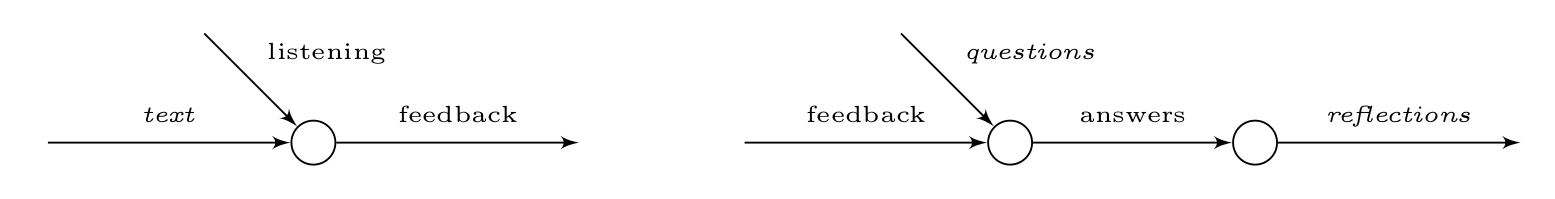
\includegraphics[width=.9\textwidth]{ww-serendipity-diagram}
%% \par}

Italicised elements (\emph{presentation}, \emph{questions}, and
\emph{reflections}) are the responsibilities of the presenting author,
and the upright elements (listening, feedback, and
answers) are the responsibilities of the attendant critics.
%
The system as a whole can be further decomposed into generative
components as follows:

\bigskip

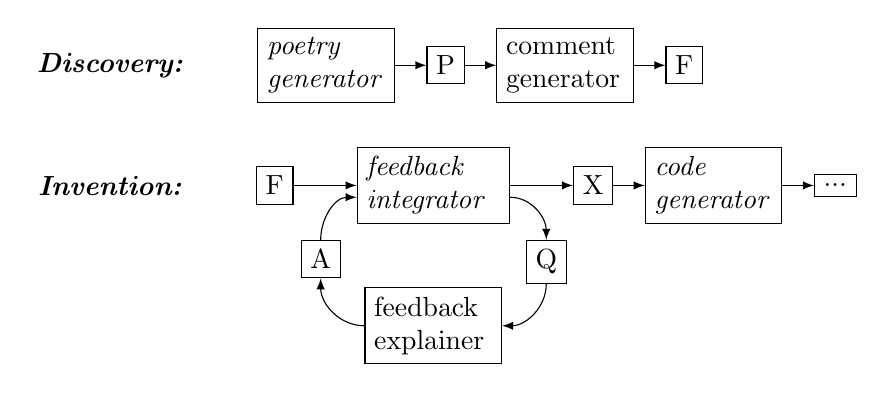
\begin{tikzpicture}[
single/.style={draw, anchor=text, rectangle},
]
\node (discovery) {\textbf{\emph{Discovery:}}};
% poet generates poem
\node[single, right=8mm of discovery.east,text width=1.5cm] (poet) {\emph{poetry generator}};
\node[single, right=4mm of poet.east] (poem) {P};
\draw [-latex] (poet.east) -- (poem.west);
% critic listens to poem and offers feedback
\node[single, right=4mm of poem.east,text width=1.5cm] (critic) {comment generator};
\draw [-latex] (poem.east) -- (critic.west);
\node[single, right=4mm of critic.east] (feedback) {F};
\draw [-latex] (critic.east) -- (feedback.west);

%%% Next phase
\node[below=1cm of discovery] (invention) {\textbf{\emph{Invention:}}};
% poet integrates feedback
\node[single, right=8mm of invention.east] (feedbackcont) {F};
\node[single, right=8mm of feedbackcont.east,text width=1.7cm] (integrator) {\emph{feedback integrator}};
\draw [-latex] (feedbackcont.east) -- (integrator.west);

\node[single, below=8mm of integrator.south,text width=1.5cm] (explainer) {feedback explainer};

\node[single, below right=2mm and 2mm of integrator] (question) {Q};
\node[single, below left=2mm and 2mm of integrator] (answer) {A};

\draw[-latex] ([yshift=-1.5mm]integrator.east) to [out=0,in=90] (question.north) ;
\draw[-latex] (question.south) to [out=270,in=0] (explainer.east) ;
\draw[-latex] (explainer.west) to [out=180,in=270] (answer.south) ;
\draw[-latex] (answer.north) to [out=90,in=180] ([yshift=-1.5mm]integrator.west) ;

\node[single, right=8mm of integrator.east] (problem) {X};

\draw [-latex] (integrator.east) -- (problem.west);

% poet reflects on feedback and updates codebase

\node[single, right=4mm of problem.east,text width=1.5cm] (pgrammer) {\emph{code}\\ \emph{generator}};

\draw [-latex] (problem.east) -- (pgrammer.west);

\node[single, right=4mm of pgrammer.east,text width=.3cm] (etc) {...};

\draw [-latex] (pgrammer.east) -- (etc.west);
\end{tikzpicture}


\bigskip

\noindent In our thought experiment, we focus on the case of hypothetical such discussions and exchange of views between computational poetry systems as our example of a situation where social circumstances could encourage serendipity. We note that similar
ideas would apply for prose and, with further adaptation, other arts.

\paragraph{Thought Experiment: Prepared mind.}
Participating systems need to be able to follow the protocol.  This
means that participating systems will need components like those
listed above. The {\tt listening} and {\tt questions} components of
the protocol correspond to $p$ and $p^{\prime}$ our model of
serendipity.  The corresponding ``comment generator'' and ``feedback
integrator'' modules in the architecture represent the primary points
of interface to the outside world.  In principle these modules need to
be prepared to deal (more or less thoughtfully) with \emph{any} text,
and in turn, with \emph{any} comment on that text.  Certain limits may
be agreed in advance; e.g.~as to genre or length in the case of texts,
and what constitutes an acceptable comment.  The ``feedback
explainer'' is closely connected with the ``comment generator'' and in
an implementation of this model they would presumably share a
codebase.  The loop for learning by asking questions as they arise is
reminiscent of the operating strategy of {\sf SHRDLU}
\cite{winograd1972understanding}.

\paragraph{Thought Experiment: Serendipity triggers.}

Although the poem is under the control of the initial generative
subsystem, it is \emph{not} under control of the listening subsystem.
The listening subsystem expects some poem, but it does not know what
poem to expect.  In this sense, the poem constitutes a serendipity
trigger $T$, not only for the listening subsystem, but for the
Workshop system as a whole.

To expand this point, note that there may be several listeners, each
sharing their own feedback and listening to the feedback presented by
others (which, again, is outside of their direct control).  This
creates further potential for serendipity, since each listener can
learn what others see in the poem.  More formally, in this case
$T^\star$ may seen as an evolving vector with shared state, but viewed
and handled from different perspectives.  With multiple agents
involved in the discussion, the ``comment generator'' module would
expand to contain its own feedback loops.

\paragraph{Thought Experiment: Bridge.}

Feedback on portions of the poem may lead the system to identify new
problems, indeed, new \emph{types} of problems that it hadn't
considered before.  The most immediately feasible case is one in which
the critic is a programmer who can directly program new concepts into
the computer \cite<cf.>{winograd1972understanding}.  However, it would
be hard to call that ``serendipity.''

We can also ask whether agents can build new concepts \emph{without}
outside intervention, starting with some basic concepts and abilities
related to poetry (e.g.~definitions of words, valence of sentiments,
metre, repetition, density, etc.) and code (e.g.~the data, functions,
and macros in which the poetic concepts and workshop protocols are
embodied).  Previous experiments with concept invention have been
fraught with questions about autonomy
\cite{ritchie1984case,lenat1984and}.  One cognitively inspired
hypothesis is that the formation of new concepts is closely related to
formation of sensory experiences \cite{milan2013kiki}.  If the
workshop participants have the capacity to identify the distinctive
features of a given poem, then training via a machine learning or
genetic algorithm approach could be used assemble a battery of
existing low-level tools that can approximate the effect.  Relatedly,
a compression process could seek to produce a given complex poetic
effect with a maximally-succinct algorithm.

The key point is that feedback on the poem -- simply describing what's
in the poem from several different points of view -- can be used to
define new problems for the system to solve.  This is not simply a
matter of decomposing the poem into pieces, but also of reconstructing
the way in which the pieces work together.  This is one of the
functions of the {\tt questions} step corresponding to $p^{\prime}$ in
our formalism: they offer the poet the opportunity to enquire about
how different pieces of feedback fit together, and learn more about
where they come from.  Although computers are currently nowhere close,
the reconstructive process may steadily approach the ideal case --
familiar to humans -- of relating to the sentiment expressed by the
poem as a whole \cite[p. 209]{bergson1983creative}.

%% Several of us are involved with a contemporary project
%% \cite{coinvent14} to develop a formal theory of concept invention,
%% focusing on \emph{concept blending}.  The additive or subtractive
%% blending of existing poetry profiles may be another way to create new
%% concepts.


%% should be possible Modifer Grammar
%% Counting Breathing Position Distribution Phonics Rhythm Repetition
%% Thematic Narrative Entropy

\paragraph{Thought Experiment: Result.} 

The final step is to take the problem or problems that were
identified, and write new code to solve them.  Several strategies for
generating a result $R$, in the form of new code, were described
above.  Now the system evaluates the new code to see whether it holds
promise.  In order to do this, it must have a way to carry out an
evaluation and judge whether $|R|>0$.  In the most straightforward
case, it would simply make changes to the draft poem that seem to
improve it in some way.  For example, the poet might remove or alter material that
elicited a negative response from a critic.  The system may proceed to
update its modules related to poetry generation.  Notably, it may also update its own
feedback modules, after reflecting on questions like: ``How might the
critic have detected that feature in my poem?''

% \section{Patterns of Serendipity} \label{sec:patterns-of-serendipity}

\begin{figure}[p]
\centering
%\input{grid-input}
\resizebox{1.0\textwidth}{!}{%
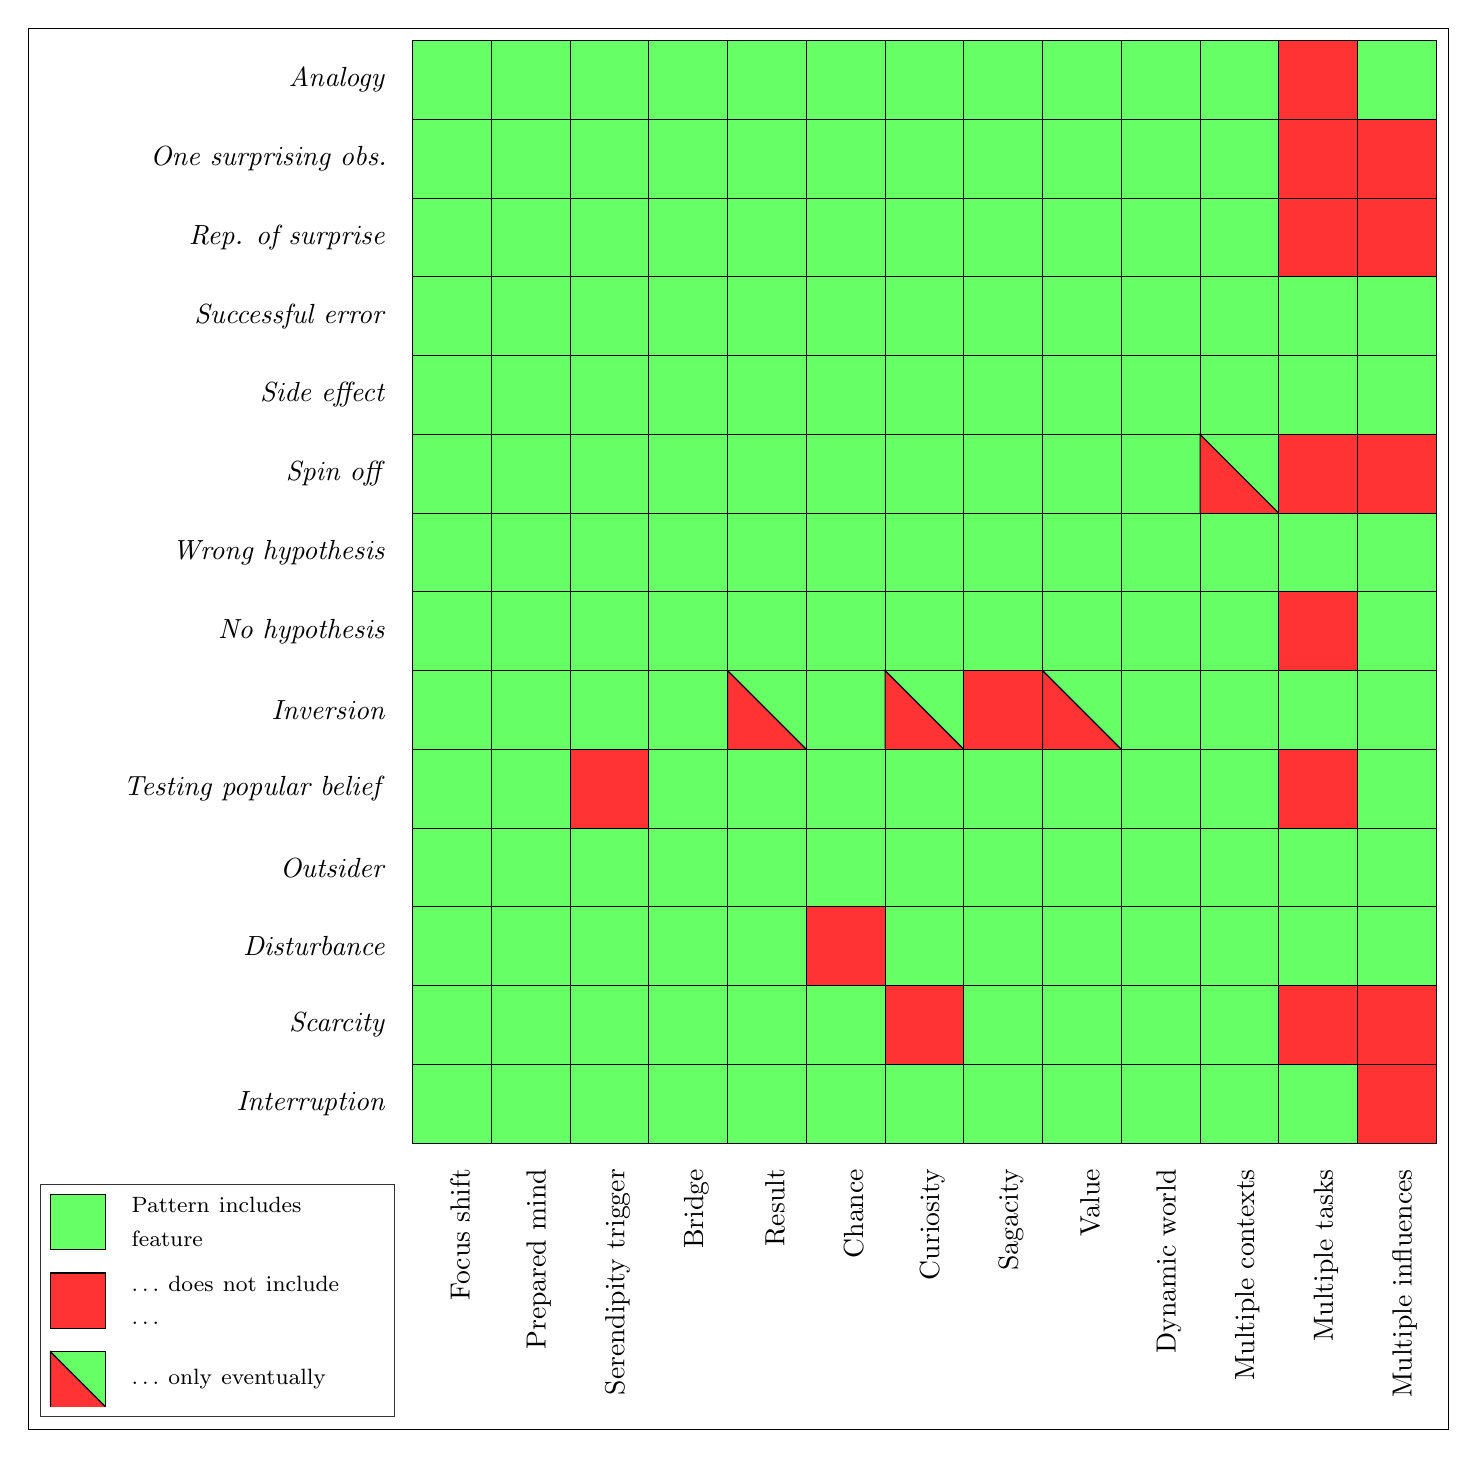
\begin{tikzpicture}[framed]
\draw[step=1cm,black,thin] (0,0) grid (12,13);
% Zeroth column
\node (bottom) at (-0.5,12.5)[draw,fill=green!60,minimum width=1cm,minimum height=1cm] {};  
\node[draw=none,left=.2cm of bottom.west,anchor=east] {\emph{Analogy}};
\node (bottom) at (-0.5,11.5)[draw,fill=green!60,minimum width=1cm,minimum height=1cm] {};  
\node[draw=none,left=.2cm of bottom.west,anchor=east] {\emph{One surprising obs.}};
\node (bottom) at (-0.5,10.5)[draw,fill=green!60,minimum width=1cm,minimum height=1cm] {};  
\node[draw=none,left=.2cm of bottom.west,anchor=east] {\emph{Rep. of surprise}};
\node (bottom) at (-0.5,9.5)[draw,fill=green!60,minimum width=1cm,minimum height=1cm] {};  
\node[draw=none,left=.2cm of bottom.west,anchor=east] {\emph{Successful error}}; 
\node (bottom) at (-0.5,8.5)[draw,fill=green!60,minimum width=1cm,minimum height=1cm] {};  
\node[draw=none,left=.2cm of bottom.west,anchor=east] {\emph{Side effect}};
\node (bottom) at (-0.5,7.5)[draw,fill=green!60,minimum width=1cm,minimum height=1cm] {};  
\node[draw=none,left=.2cm of bottom.west,anchor=east] {\emph{Spin off}};
\node (bottom) at (-0.5,6.5)[draw,fill=green!60,minimum width=1cm,minimum height=1cm] {};  
\node[draw=none,left=.2cm of bottom.west,anchor=east] {\emph{Wrong hypothesis}};
\node (bottom) at (-0.5,5.5)[draw,fill=green!60,minimum width=1cm,minimum height=1cm] {};  
\node[draw=none,left=.2cm of bottom.west,anchor=east] {\emph{No hypothesis}};
\node (bottom) at (-0.5,4.5)[draw,fill=green!60,minimum width=1cm,minimum height=1cm] {};  
\node[draw=none,left=.2cm of bottom.west,anchor=east] {\emph{Inversion}};
\node (bottom) at (-0.5,3.5)[draw,fill=green!60,minimum width=1cm,minimum height=1cm] {};  
\node[draw=none,left=.2cm of bottom.west,anchor=east] {\emph{Testing popular belief}};
\node (bottom) at (-0.5,2.5)[draw,fill=green!60,minimum width=1cm,minimum height=1cm] {};  
\node[draw=none,left=.2cm of bottom.west,anchor=east] {\emph{Outsider}};
\node (bottom) at (-0.5,1.5)[draw,fill=green!60,minimum width=1cm,minimum height=1cm] {};  
\node[draw=none,left=.2cm of bottom.west,anchor=east] {\emph{Disturbance}};
\node (bottom) at (-0.5,0.5)[draw,fill=green!60,minimum width=1cm,minimum height=1cm] {};  
\node[draw=none,left=.2cm of bottom.west,anchor=east] {\emph{Scarcity}}; 
\node (bottom) at (-0.5,-0.5)[draw,fill=green!60,minimum width=1cm,minimum height=1cm] {};  
\node[draw=none,left=.2cm of bottom.west,anchor=east] {\emph{Interruption}};
\node[draw=none,rotate=90,below=.2cm of bottom.south,yshift=-.1cm,anchor=east] {Focus shift};
% First column
\node (bottom) at (0.5,12.5)[draw,fill=green!60,minimum width=1cm,minimum height=1cm] {};  
\node (bottom) at (0.5,11.5)[draw,fill=green!60,minimum width=1cm,minimum height=1cm] {};  
\node (bottom) at (0.5,10.5)[draw,fill=green!60,minimum width=1cm,minimum height=1cm] {};  
\node (bottom) at (0.5,9.5)[draw,fill=green!60,minimum width=1cm,minimum height=1cm] {};  
\node (bottom) at (0.5,8.5)[draw,fill=green!60,minimum width=1cm,minimum height=1cm] {};  
\node (bottom) at (0.5,7.5)[draw,fill=green!60,minimum width=1cm,minimum height=1cm] {};  
\node (bottom) at (0.5,6.5)[draw,fill=green!60,minimum width=1cm,minimum height=1cm] {};  
\node (bottom) at (0.5,5.5)[draw,fill=green!60,minimum width=1cm,minimum height=1cm] {};  
\node (bottom) at (0.5,4.5)[draw,fill=green!60,minimum width=1cm,minimum height=1cm] {};  
\node (bottom) at (0.5,3.5)[draw,fill=green!60,minimum width=1cm,minimum height=1cm] {};  
\node (bottom) at (0.5,2.5)[draw,fill=green!60,minimum width=1cm,minimum height=1cm] {};  
\node (bottom) at (0.5,1.5)[draw,fill=green!60,minimum width=1cm,minimum height=1cm] {};  
\node (bottom) at (0.5,0.5)[draw,fill=green!60,minimum width=1cm,minimum height=1cm] {};  
\node (bottom) at (0.5,-0.5)[draw,fill=green!60,minimum width=1cm,minimum height=1cm] {};  
\node[draw=none,rotate=90,below=.2cm of bottom.south,yshift=-.1cm,anchor=east] {Prepared mind};
 % Interruption               
% Second column
\node at (1.5,12.5) [draw,fill=green!60,minimum width=1cm,minimum height=1cm]{};
\node at (1.5,11.5) [draw,fill=green!60,minimum width=1cm,minimum height=1cm]{};
\node at (1.5,10.5) [draw,fill=green!60,minimum width=1cm,minimum height=1cm]{};
\node at (1.5,9.5)  [draw,fill=green!60,minimum width=1cm,minimum height=1cm]{};
\node at (1.5,8.5)  [draw,fill=green!60,minimum width=1cm,minimum height=1cm]{};
\node at (1.5,7.5)  [draw,fill=green!60,minimum width=1cm,minimum height=1cm]{};
\node at (1.5,6.5)  [draw,fill=green!60,minimum width=1cm,minimum height=1cm]{};
\node at (1.5,5.5)  [draw,fill=green!60,minimum width=1cm,minimum height=1cm]{};
\node at (1.5,4.5)  [draw,fill=green!60,minimum width=1cm,minimum height=1cm]{};
\node at (1.5,3.5)  [draw,fill=red!80,minimum width=1cm,minimum height=1cm]{};
\node at (1.5,2.5)  [draw,fill=green!60,minimum width=1cm,minimum height=1cm]{};
\node at (1.5,1.5)  [draw,fill=green!60,minimum width=1cm,minimum height=1cm]{};
\node at (1.5,0.5)  [draw,fill=green!60,minimum width=1cm,minimum height=1cm]{};
\node (bottom) at (1.5,-0.5)[draw,fill=green!60,minimum width=1cm,minimum height=1cm] {};  
\node[draw=none,rotate=90,below=.2cm of bottom.south,yshift=-.1cm,anchor=east] {Serendipity trigger};
% Third column
\node at (2.5,12.5) [draw,fill=green!60,minimum width=1cm,minimum height=1cm]{}; % Analogy                    
\node at (2.5,11.5) [draw,fill=green!60,minimum width=1cm,minimum height=1cm]{}; % One surprising observation 
\node at (2.5,10.5) [draw,fill=green!60,minimum width=1cm,minimum height=1cm]{}; % Repetition of surprise     
\node at (2.5,9.5)  [draw,fill=green!60,minimum width=1cm,minimum height=1cm]{}; % Successful error           
\node at (2.5,8.5)  [draw,fill=green!60,minimum width=1cm,minimum height=1cm]{}; % Side effect                
\node at (2.5,7.5)  [draw,fill=green!60,minimum width=1cm,minimum height=1cm]{}; % Spin off                   
\node at (2.5,6.5)  [draw,fill=green!60,minimum width=1cm,minimum height=1cm]{}; % Wrong hypothesis           
\node at (2.5,5.5)  [draw,fill=green!60,minimum width=1cm,minimum height=1cm]{}; % No hypothesis              
\node at (2.5,4.5)  [draw,fill=green!60,minimum width=1cm,minimum height=1cm]{}; % Inversion                  
\node at (2.5,3.5)  [draw,fill=green!60,minimum width=1cm,minimum height=1cm]{}; % Testing popular belief     
\node at (2.5,2.5)  [draw,fill=green!60,minimum width=1cm,minimum height=1cm]{}; % outsider    
\node at (2.5,1.5)  [draw,fill=green!60,minimum width=1cm,minimum height=1cm]{}; % Disturbance                
\node at (2.5,0.5)  [draw,fill=green!60,minimum width=1cm,minimum height=1cm]{}; % Scarcity                   
\node (bottom) at (2.5,-0.5)[draw,fill=green!60,minimum width=1cm,minimum height=1cm] {};  
\node[draw=none,rotate=90,below=.2cm of bottom.south,yshift=-.1cm,anchor=east] {Bridge};
% Fourth column
\node at (3.5,12.5) [draw,fill=green!60,minimum width=1cm,minimum height=1cm]{}; % Analogy                    
\node at (3.5,11.5) [draw,fill=green!60,minimum width=1cm,minimum height=1cm]{}; % One surprising observation 
\node at (3.5,10.5) [draw,fill=green!60,minimum width=1cm,minimum height=1cm]{}; % Repetition of surprise     
\node at (3.5,9.5)  [draw,fill=green!60,minimum width=1cm,minimum height=1cm]{}; % Successful error           
\node at (3.5,8.5)  [draw,fill=green!60,minimum width=1cm,minimum height=1cm]{}; % Side effect                
\node at (3.5,7.5)  [draw,fill=green!60,minimum width=1cm,minimum height=1cm]{}; % Spin off                   
\node at (3.5,6.5)  [draw,fill=green!60,minimum width=1cm,minimum height=1cm]{}; % Wrong hypothesis           
\node at (3.5,5.5)  [draw,fill=green!60,minimum width=1cm,minimum height=1cm]{}; % No hypothesis              
\node at (3.5,4.5)  [draw,fill=green!60,minimum width=1cm,minimum height=1cm]{}; % Inversion
\draw [fill=red!80] (3,4) -- (3,5) -- (4,4);  
\node at (3.5,3.5)  [draw,fill=green!60,minimum width=1cm,minimum height=1cm]{}; % Testing popular belief     
\node at (3.5,2.5)  [draw,fill=green!60,minimum width=1cm,minimum height=1cm]{}; % Outsider
\node at (3.5,1.5)  [draw,fill=green!60,minimum width=1cm,minimum height=1cm]{}; % Disturbance                
\node at (3.5,0.5)  [draw,fill=green!60,minimum width=1cm,minimum height=1cm]{}; % Scarcity                   
%\node at (3,0)  [draw,fill=green!60,minimum width=1cm,minimum height=1cm]{}; % Interruption               
\node (bottom) at (3.5,-0.5)[draw,fill=green!60,minimum width=1cm,minimum height=1cm] {};  
\node[draw=none,rotate=90,below=.2cm of bottom.south,yshift=-.1cm,anchor=east] {Result};
% Fifth column
\node at (4.5,12.5) [draw,fill=green!60,minimum width=1cm,minimum height=1cm]{}; % Analogy                    
\node at (4.5,11.5) [draw,fill=green!60,minimum width=1cm,minimum height=1cm]{}; % One surprising observation 
\node at (4.5,10.5) [draw,fill=green!60,minimum width=1cm,minimum height=1cm]{}; % Repetition of surprise     
\node at (4.5,9.5)  [draw,fill=green!60,minimum width=1cm,minimum height=1cm]{}; % Successful error           
\node at (4.5,8.5)  [draw,fill=green!60,minimum width=1cm,minimum height=1cm]{}; % Side effect                
\node at (4.5,7.5)  [draw,fill=green!60,minimum width=1cm,minimum height=1cm]{}; % Spin off                   
\node at (4.5,6.5)  [draw,fill=green!60,minimum width=1cm,minimum height=1cm]{}; % Wrong hypothesis           
\node at (4.5,5.5)  [draw,fill=green!60,minimum width=1cm,minimum height=1cm]{}; % No hypothesis              
\node at (4.5,4.5)  [draw,fill=green!60,minimum width=1cm,minimum height=1cm]{}; % Inversion
\node at (4.5,3.5)  [draw,fill=green!60,minimum width=1cm,minimum height=1cm]{}; % Testing popular belief     
\node at (4.5,2.5)  [draw,fill=green!60,minimum width=1cm,minimum height=1cm]{}; % Testing popular belief     
\node at (4.5,1.5)  [draw,fill=red!80,minimum width=1cm,minimum height=1cm]{}; % Disturbance                
\node at (4.5,0.5)  [draw,fill=green!60,minimum width=1cm,minimum height=1cm]{}; % Scarcity                   
% \node at (4,0)  [draw,fill=green!60,minimum width=1cm,minimum height=1cm]{}; % Interruption               
\node (bottom) at (4.5,-0.5)[draw,fill=green!60,minimum width=1cm,minimum height=1cm] {};  
\node[draw=none,rotate=90,below=.2cm of bottom.south,yshift=-.1cm,anchor=east] {Chance};
% Sixth column
\node at (5.5,12.5) [draw,fill=green!60,minimum width=1cm,minimum height=1cm]{}; % Analogy                    
\node at (5.5,11.5) [draw,fill=green!60,minimum width=1cm,minimum height=1cm]{}; % One surprising observation 
\node at (5.5,10.5) [draw,fill=green!60,minimum width=1cm,minimum height=1cm]{}; % Repetition of surprise     
\node at (5.5,9.5)  [draw,fill=green!60,minimum width=1cm,minimum height=1cm]{}; % Successful error           
\node at (5.5,8.5)  [draw,fill=green!60,minimum width=1cm,minimum height=1cm]{}; % Side effect                
\node at (5.5,7.5)  [draw,fill=green!60,minimum width=1cm,minimum height=1cm]{}; % Spin off                   
\node at (5.5,6.5)  [draw,fill=green!60,minimum width=1cm,minimum height=1cm]{}; % Wrong hypothesis           
\node at (5.5,5.5)  [draw,fill=green!60,minimum width=1cm,minimum height=1cm]{}; % No hypothesis              
\node at (5.5,4.5)  [draw,fill=green!60,minimum width=1cm,minimum height=1cm]{}; % Inversion                  
\draw [fill=red!80] (5,4) -- (5,5) -- (6,4);  
\node at (5.5,3.5)  [draw,fill=green!60,minimum width=1cm,minimum height=1cm]{}; % Testing popular belief     
\node at (5.5,2.5)  [draw,fill=green!60,minimum width=1cm,minimum height=1cm]{}; % Testing popular belief     
\node at (5.5,1.5)  [draw,fill=green!60,minimum width=1cm,minimum height=1cm]{}; % Disturbance                
\node at (5.5,0.5)  [draw,fill=red!80,minimum width=1cm,minimum height=1cm]{}; % Scarcity                   
% \node at (5,0)  [draw,fill=green!60,minimum width=1cm,minimum height=1cm]{}; % Interruption               
\node (bottom) at (5.5,-0.5)[draw,fill=green!60,minimum width=1cm,minimum height=1cm] {};  
\node[draw=none,rotate=90,below=.2cm of bottom.south,yshift=-.1cm,anchor=east] {Curiosity};
% Seventh column
\node at (6.5,12.5) [draw,fill=green!60,minimum width=1cm,minimum height=1cm]{}; % Analogy                    
\node at (6.5,11.5) [draw,fill=green!60,minimum width=1cm,minimum height=1cm]{}; % One surprising observation 
\node at (6.5,10.5) [draw,fill=green!60,minimum width=1cm,minimum height=1cm]{}; % Repetition of surprise     
\node at (6.5,9.5)  [draw,fill=green!60,minimum width=1cm,minimum height=1cm]{}; % Successful error           
\node at (6.5,8.5)  [draw,fill=green!60,minimum width=1cm,minimum height=1cm]{}; % Side effect                
\node at (6.5,7.5)  [draw,fill=green!60,minimum width=1cm,minimum height=1cm]{}; % Spin off                   
\node at (6.5,6.5)  [draw,fill=green!60,minimum width=1cm,minimum height=1cm]{}; % Wrong hypothesis           
\node at (6.5,5.5)  [draw,fill=green!60,minimum width=1cm,minimum height=1cm]{}; % No hypothesis              
\node at (6.5,4.5)  [draw,fill=red!80,minimum width=1cm,minimum height=1cm]{}; % Inversion                  
\node at (6.5,3.5)  [draw,fill=green!60,minimum width=1cm,minimum height=1cm]{}; % Testing popular belief     
\node at (6.5,2.5)  [draw,fill=green!60,minimum width=1cm,minimum height=1cm]{}; % Testing popular belief     
\node at (6.5,1.5)  [draw,fill=green!60,minimum width=1cm,minimum height=1cm]{}; % Disturbance                
\node at (6.5,0.5)  [draw,fill=green!60,minimum width=1cm,minimum height=1cm]{}; % Scarcity                   
% \node at (6,0)  [draw,fill=green!60,minimum width=1cm,minimum height=1cm]{}; % Interruption               
\node (bottom) at (6.5,-0.5)[draw,fill=green!60,minimum width=1cm,minimum height=1cm] {};  
\node[draw=none,rotate=90,below=.2cm of bottom.south,yshift=-.1cm,anchor=east] {Sagacity};
% Eighth column
\node at (7.5,12.5) [draw,fill=green!60,minimum width=1cm,minimum height=1cm]{}; % Analogy                    
\node at (7.5,11.5) [draw,fill=green!60,minimum width=1cm,minimum height=1cm]{}; % One surprising observation 
\node at (7.5,10.5) [draw,fill=green!60,minimum width=1cm,minimum height=1cm]{}; % Repetition of surprise     
\node at (7.5,9.5)  [draw,fill=green!60,minimum width=1cm,minimum height=1cm]{}; % Successful error           
\node at (7.5,8.5)  [draw,fill=green!60,minimum width=1cm,minimum height=1cm]{}; % Side effect                
\node at (7.5,7.5)  [draw,fill=green!60,minimum width=1cm,minimum height=1cm]{}; % Spin off                   
\node at (7.5,6.5)  [draw,fill=green!60,minimum width=1cm,minimum height=1cm]{}; % Wrong hypothesis           
\node at (7.5,5.5)  [draw,fill=green!60,minimum width=1cm,minimum height=1cm]{}; % No hypothesis              
%\node at (7.5,4.5)  [draw,shading=axis,bottom color=green!60,top color=red,minimum width=1cm,minimum height=1cm,shading angle=45]{}; % Inversion
\node at (7.5,4.5)  [draw,fill=green!60,minimum width=1cm,minimum height=1cm]{}; % Inversion
%% half off
\draw [fill=red!80] (7,4) -- (7,5) -- (8,4);  % Interruption
%\draw (7,4) -- (8,5);  % Interruption
\node at (7.5,3.5)  [draw,fill=green!60,minimum width=1cm,minimum height=1cm]{}; % Testing popular belief     
\node at (7.5,2.5)  [draw,fill=green!60,minimum width=1cm,minimum height=1cm]{}; % outsider
\node at (7.5,1.5)  [draw,fill=green!60,minimum width=1cm,minimum height=1cm]{}; % Disturbance                
\node at (7.5,0.5)  [draw,fill=green!60,minimum width=1cm,minimum height=1cm]{}; % Scarcity                   
%\node at (7,0)  [draw,fill=green!60,minimum width=1cm,minimum height=1cm]{}; % Interruption               
\node (bottom) at (7.5,-0.5)[draw,fill=green!60,minimum width=1cm,minimum height=1cm] {};  
\node[draw=none,rotate=90,below=.2cm of bottom.south,yshift=-.1cm,anchor=east] {Value};
%%%%%%%%%%%%%%%
% Ninth column
\node at (8.5,12.5) [draw,fill=green!60,minimum width=1cm,minimum height=1cm]{}; % Analogy                    
\node at (8.5,11.5) [draw,fill=green!60,minimum width=1cm,minimum height=1cm]{}; % One surprising observation 
\node at (8.5,10.5) [draw,fill=green!60,minimum width=1cm,minimum height=1cm]{}; % Repetition of surprise     
\node at (8.5,9.5)  [draw,fill=green!60,minimum width=1cm,minimum height=1cm]{}; % Successful error           
\node at (8.5,8.5)  [draw,fill=green!60,minimum width=1cm,minimum height=1cm]{}; % Side effect                
\node at (8.5,7.5)  [draw,fill=green!60,minimum width=1cm,minimum height=1cm]{}; % Spin off                   
\node at (8.5,6.5)  [draw,fill=green!60,minimum width=1cm,minimum height=1cm]{}; % Wrong hypothesis           
\node at (8.5,5.5)  [draw,fill=green!60,minimum width=1cm,minimum height=1cm]{}; % No hypothesis              
\node at (8.5,4.5)  [draw,fill=green!60,minimum width=1cm,minimum height=1cm]{}; % Inversion                  
\node at (8.5,3.5)  [draw,fill=green!60,minimum width=1cm,minimum height=1cm]{}; % Testing popular belief     
\node at (8.5,2.5)  [draw,fill=green!60,minimum width=1cm,minimum height=1cm]{}; % Testing popular belief     
\node at (8.5,1.5)  [draw,fill=green!60,minimum width=1cm,minimum height=1cm]{}; % Disturbance                
\node at (8.5,0.5)  [draw,fill=green!60,minimum width=1cm,minimum height=1cm]{}; % Scarcity                   
% \node at (8,0)  [draw,fill=green!60,minimum width=1cm,minimum height=1cm]{}; % Interruption               
\node (bottom) at (8.5,-0.5)[draw,fill=green!60,minimum width=1cm,minimum height=1cm] {};  
\node[draw=none,rotate=90,below=.2cm of bottom.south,yshift=-.1cm,anchor=east] {Dynamic world};
% Tenth column
\node at (9.5,12.5) [draw,fill=green!60,minimum width=1cm,minimum height=1cm]{}; % Analogy                    
\node at (9.5,11.5) [draw,fill=green!60,minimum width=1cm,minimum height=1cm]{}; % One surprising observation 
\node at (9.5,10.5) [draw,fill=green!60,minimum width=1cm,minimum height=1cm]{}; % Repetition of surprise     
\node at (9.5,9.5)  [draw,fill=green!60,minimum width=1cm,minimum height=1cm]{}; % Successful error           
\node at (9.5,8.5)  [draw,fill=green!60,minimum width=1cm,minimum height=1cm]{}; % Side effect                
\node at (9.5,7.5)  [draw,fill=green!60,minimum width=1cm,minimum height=1cm]{}; % Spin off
\draw [fill=red!80] (9,7) -- (9,8) -- (10,7);  
\node at (9.5,6.5)  [draw,fill=green!60,minimum width=1cm,minimum height=1cm]{}; % Wrong hypothesis           
\node at (9.5,5.5)  [draw,fill=green!60,minimum width=1cm,minimum height=1cm]{}; % No hypothesis              
\node at (9.5,4.5)  [draw,fill=green!60,minimum width=1cm,minimum height=1cm]{}; % Inversion                  
\node at (9.5,3.5)  [draw,fill=green!60,minimum width=1cm,minimum height=1cm]{}; % Testing popular belief     
\node at (9.5,2.5)  [draw,fill=green!60,minimum width=1cm,minimum height=1cm]{}; % Testing popular belief     
\node at (9.5,1.5)  [draw,fill=green!60,minimum width=1cm,minimum height=1cm]{}; % Disturbance                
\node at (9.5,0.5)  [draw,fill=green!60,minimum width=1cm,minimum height=1cm]{}; % Scarcity                   
% \node at (9,0)  [draw,fill=green!60,minimum width=1cm,minimum height=1cm]{}; % Interruption               
\node (bottom) at (9.5,-0.5)[draw,fill=green!60,minimum width=1cm,minimum height=1cm] {};  
\node[draw=none,rotate=90,below=.2cm of bottom.south,yshift=-.1cm,anchor=east] {Multiple contexts};
% Eleventh column
\node at (10.5,12.5) [draw,fill=red!80,minimum width=1cm,minimum height=1cm]{}; % Analogy                    
\node at (10.5,11.5) [draw,fill=red!80,minimum width=1cm,minimum height=1cm]{}; % One surprising observation 
\node at (10.5,10.5) [draw,fill=red!80,minimum width=1cm,minimum height=1cm]{}; % Repetition of surprise     
\node at (10.5,9.5)  [draw,fill=green!60,minimum width=1cm,minimum height=1cm]{}; % Successful error           
\node at (10.5,8.5)  [draw,fill=green!60,minimum width=1cm,minimum height=1cm]{}; % Side effect                
\node at (10.5,7.5)  [draw,fill=red!80,minimum width=1cm,minimum height=1cm]{}; % Spin off                   
\node at (10.5,6.5)  [draw,fill=green!60,minimum width=1cm,minimum height=1cm]{}; % Wrong hypothesis           
\node at (10.5,5.5)  [draw,fill=red!80,minimum width=1cm,minimum height=1cm]{}; % No hypothesis              
\node at (10.5,4.5)  [draw,fill=green!60,minimum width=1cm,minimum height=1cm]{}; % Inversion                  
\node at (10.5,3.5)  [draw,fill=red!80,minimum width=1cm,minimum height=1cm]{}; % Testing popular belief     
\node at (10.5,2.5)  [draw,fill=green!60,minimum width=1cm,minimum height=1cm]{}; % outsider
\node at (10.5,1.5)  [draw,fill=green!60,minimum width=1cm,minimum height=1cm]{}; % Disturbance                
\node at (10.5,0.5)  [draw,fill=red!80,minimum width=1cm,minimum height=1cm]{}; % Scarcity                   
% \node at (10,0)  [draw,fill=green!60,minimum width=1cm,minimum height=1cm]{}; % Interruption               
\node (bottom) at (10.5,-0.5)[draw,fill=green!60,minimum width=1cm,minimum height=1cm] {};  
\node[draw=none,rotate=90,below=.2cm of bottom.south,yshift=-.1cm,anchor=east] {Multiple tasks};
% Twelfth column
\node at (11.5,12.5) [draw,fill=green!60,minimum width=1cm,minimum height=1cm]{}; % Analogy                    
\node at (11.5,11.5) [draw,fill=red!80,minimum width=1cm,minimum height=1cm]{}; % One surprising observation 
\node at (11.5,10.5) [draw,fill=red!80,minimum width=1cm,minimum height=1cm]{}; % Repetition of surprise     
\node at (11.5,9.5)  [draw,fill=green!60,minimum width=1cm,minimum height=1cm]{}; % Successful error           
\node at (11.5,8.5)  [draw,fill=green!60,minimum width=1cm,minimum height=1cm]{}; % Side effect                
\node at (11.5,7.5)  [draw,fill=red!80,minimum width=1cm,minimum height=1cm]{}; % Spin off                   
\node at (11.5,6.5)  [draw,fill=green!60,minimum width=1cm,minimum height=1cm]{}; % Wrong hypothesis           
\node at (11.5,5.5)  [draw,fill=green!60,minimum width=1cm,minimum height=1cm]{}; % No hypothesis              
\node at (11.5,4.5)  [draw,fill=green!60,minimum width=1cm,minimum height=1cm]{}; % Inversion                  
\node at (11.5,3.5)  [draw,fill=green!60,minimum width=1cm,minimum height=1cm]{}; % Testing popular belief     
\node at (11.5,2.5)  [draw,fill=green!60,minimum width=1cm,minimum height=1cm]{}; % Testing popular belief     
\node at (11.5,1.5)  [draw,fill=green!60,minimum width=1cm,minimum height=1cm]{}; % Disturbance                
\node at (11.5,0.5)  [draw,fill=red!80,minimum width=1cm,minimum height=1cm]{}; % Scarcity                   
\node (bottom) at (11.5,-0.5)[draw,fill=red!80,minimum width=1cm,minimum height=1cm] {};  
\node[draw=none,rotate=90,below=.2cm of bottom.south,yshift=-.1cm,anchor=east] {Multiple influences};

\begin{scope}[xshift=.5cm,yshift=0cm]
\node (A) at (-5.75,-2.0)  [draw,fill=green!60,minimum width=.7cm,minimum height=.7cm]{}; %
\node[draw=none,right=.2cm of A.east,text width=3.10cm] {{\footnotesize Pattern includes\par feature}}; 
\node (B) at (-5.75,-3.0)  [draw,fill=red!80,minimum width=.7cm,minimum height=.7cm]{}; %
\node[draw=none,right=.2cm of B.east,text width=3.10cm] {{\footnotesize $\ldots$ does not include $\ldots$}}; 

\node (C) at (-5.75,-4)  [draw,fill=green!60,minimum width=.7cm,minimum height=.7cm]{}; %
\node[draw=none,right=.2cm of C.east,text width=3.10cm] (Ct) {{\footnotesize $\ldots$ only eventually}};
%% half off
\draw [fill=red!80] (-6.1,-4.35) -- (-6.1,-3.65) -- (-5.4,-4.35);  

\node[draw=black!80, fit=(A) (B) (C) (Ct)](FIt1) {};
\end{scope}
\end{tikzpicture}
}
\caption{Characteristics of Pek van Andel's patterns of serendipity\label{fig:grid}}
\end{figure}

% ***AJ what is a 'situational pattern of serendipity'? Can we add a definition e.g. from van Andel***
Figure \ref{fig:grid} examines 14 situational patterns of serendipity
collected by van Andel \cite{van1994anatomy} through the lens of the evaluation
criteria described in Section \ref{sec:literature-review}.
%
As required by our theory, a ``focus shift'' appears in each instance,
although it has a different flavour in the different examples.  In
this analysis, only three of the other criteria mentioned above are
clearly present in \emph{all} of the patterns: ``a prepared mind'', a
``bridge'', and a ``dynamic world.''  Similarly, only four of van
Andel's patterns exhibit all of the characteristics we identified:
\emph{Successful error}, \emph{Side effect}, \emph{Wrong hypothesis},
and \emph{Outsider}.

``Near misses'' are also of interest, and help to illustrate the role
of the various factors from Section \ref{sec:literature-review}.
%
For example, the \emph{Inversion} pattern is somewhat closer to what is called an \emph{antipattern} in the design pattern literature \cite{brown1998antipatterns}.  Van Andel describes the story of a researcher observing an effect (the anticoagulant heparine) which was precisely the opposite of the one sought (factors that \emph{cause} blood clotting) -- and failing to acknowledge that this observation was important for over 40 years.  The result was eventually seen to be of value: however, in this instance, we may have an example of a mind that is \emph{over-prepared}, and focused on a particular sort of result, rather than a truly ``sagacious'' mind that is both prepared and open to serendipitous findings.

In the case of \emph{Testing popular belief}, van Andel gives an
account of a medical practise that originated in a folk claim, namely
cowpox-derived immunity to smallpox.  This effect, for milkmaids,
might indeed be called serendipitous.  Indeed, the medical use of
cowpox has been described as ``widely know'' \cite{riedel2005edward}
prior to its popularisation by Edward Jenner.  Nevertheless, 
Jenner's ``relentless promotion and devoted research of vaccination
\ldots changed the way medicine was practised'' \cite{riedel2005edward}.
This again might be called serendipity, but most clearly at the social
rather than personal level.  These comments should not be seen to
disparage Jenner's contribution, or diminish the role of a curious
chain of events in his personal history that tied his fate to that of
the smallpox vaccine.  Many of these had the air of serendipity about
them -- but even so, it is hard to find one specific ``serendipity
trigger.''
 
In describing \emph{Disturbance}, van Andel's exemplar is the
creation of radio telescopy from noise in transatlantic telephone calls
(paralleling the subsequent discovery by Penzias and Wilson).  Here it
is hard to see an overt role for ``chance,'' since as machinery at
various scales is created, disturbance is somewhat inevitable, even if
a specific disturbance in a specific machine is unexpected.
Similarly, in cases of \emph{Scarcity}, ``curiosity'' may not play a
significant role, and may instead be replaced by the drive of desire
and corresponding ingenuity.

Multiple contexts, tasks, and influences should be seen to be
conducive to serendipitous discovery, but not strictly necessary.  For
example, in addition to the context of a research laboratory, there
may be the context of subsequent industrial application.  However,
within the laboratory itself (where a \emph{Spin off} discovery might
be made) the future context is not typically in force.

There are a number of additional reoccurring themes, which are worthy
of further comment, and which could form the basis of further
(meta-)patterns.

\begin{description}
\item[\emph{It's all part of a day's work.}] Often the discoverer had
  a problem to solve or job to do, and made the serendipitous
  discovery in the course of doing their job.  This sort of
  serendipity is often ``social.''  For example, in the
  \emph{Outsider} pattern, the ophthalmologist Gregg was simply
  listening to his patient and taking what she said seriously; in
  other words, he was doing his job.  But this led to a new
  hypothesis.
\item[\emph{Factorisation is useful.}] Variability, and in the case of
  scientific work, factorisation (e.g. via control studies) often
  plays a key role in establishing ``multiple contexts.''
  Serendipitous discovery often happens in the context of ``natural
  experiments,'' for example, in the case of \emph{One surprising
    observation}, where van Andel's example dealt with the observation
  that one tree in a row was taller and healthier than its
  neighbours.\footnote{Concerning the broader issues associated with
    the ``design'' of such experiments, see
    \cite{imbens1994identification}.}
\item[\emph{A good story is liable to change.}] Comparing
  \emph{Inversion} and \emph{Spin off} suggests the value of being
  able to change the story.  If Perkin had suppressed his discovery of
  mauvine because he hadn't successfully synthesised quinine, there
  would have been no spin off, and it would be hard to call the
  discovery ``serendipitous'' -- or, indeed, to consider it to be a
  discovery at all.  Whatever its value, an event may only be
  \emph{described} as serendipitous at the narrative level.
\item[\emph{Watch out for hidden symmetries.}] The \emph{Wrong
  hypothesis} pattern involves several of the points above.  In van
  Andel's anecdote about John Cade's discovery of lithium as a
  \emph{treatment} for mania, the issues under investigation were,
  rather, the \emph{causes} of the illness.  This was initially
  conceptualised in terms of \emph{surfeit} and \emph{deficiency}.  A
  more general interpretation is that the factors influencing the
  course of an illness have hidden interactions between them.
  Serendipitous discovery may be able to find and capitalise on this
  type of (unexpected) invariant.
\end{description}

Van Andel describes three additional patterns that seem to be
connected with personal qualities of the investigator rather than with
situational features.  These are \emph{Playing}, \emph{Joke}, and
\emph{Dream}.  The theme of personal qualities and skills that support
serendipitous discovery will be taken up below, as part of a general
approach to modelling serendipity.

\subsection{Modelling serendipity with design patterns} \label{sec:unified-approach}

As illustrated above, serendipity can take place on multiple scales.
Something can be personally surprising while being socially mundane
(Boden's \emph{P-creativity} \cite{boden}), or vice versa, as in
the case of personally mundane discoveries that take on surprising
social value.

In the case of serendipitous discoveries at the personal level, the
qualities of the investigator are understood to be important features.
Thus, for example, van Andel writes that a ``sense of humour and
  sense of serendipity have a lot in common.'' 
% 
Van Andel relates the \emph{Dream} pattern -- exemplified, for him by
Descartes, but Kekul\'e's ouroborus provides another instance -- to
Poincar\'e's \cite{poincare1910creation,poincare2013science} model of
``preparation, incubation, illumination, and verification''
(cf. \cite{wallas1926art}).  Poincar\'e \cite{poincare1910creation}
clarifies that
\begin{quote}
``\emph{unconscious work}~\ldots~\emph{is possible, and of a
    certainty, it is only fruitful, if it is on the one hand preceded
    and on the other hand followed by a period of conscious work.}''
\end{quote}

What might conceptions like this mean for serendipity that takes place
on a social or indeed computational level?  In order to understand
this, we will refer van Andel's patterns and the serendipity factors
introduced above to the heterodox theory of patterns coming from the
field of design, mentioned briefly above.  First introduced by the
architect Christopher Alexander
\cite{alexander1979timeless,alexander1977pattern}, the design pattern
methodology spread from architecture to software
\cite{gabriel1996patterns}, and later, to other fields, including
public affairs \cite{schuler2008liberating} and education
\cite{bergin2012pedagogical}.

Alexander's patterns are presented in a tree-like structure called a
\emph{pattern language}, ordered in a top-down manner from large-scale
to small-scale levels of application, with each pattern presented in
terms of a \emph{picture}, a \emph{context} (including links to
relevant larger patterns), the \emph{problem} that the pattern
addresses, the \emph{solution}, a \emph{diagram}, and \emph{links to
  smaller patterns} \cite[pp. x-xi]{alexander1977pattern}.
%
A relatively convincing implementation of
Alexander's idea of patterns as a ``living
  language''
\cite[p. xvii]{alexander1977pattern} was realised
with one of the earliest applications of wiki
software developed by Ward Cunningham: the
Portland Pattern
Repository.\footnote{\url{http://c2.com/ppr/}}
The notion of pattern-finding as a process
related to, but distinct from abstraction, is
described by Richard Gabriel, who emphasises that
the ``patterns and the social process for
  applying them are designed to produce organic
  order through piecemeal growth''
\cite[p. 31]{gabriel1996patterns}.
%
In its original form, this statement describes the generative use of
patterns to create artefacts (buildings, object oriented programs,
etc.).  However, this criterion can also be applied to the growth and
development the pattern language itself, and this is the key idea
underlying our application.

Christian Kohls \cite{kohls2010structure,kohls2011structure}, deploys
a ``path'' or ``journey'' metaphor to describe design patterns in the
language of constrained optimisation problems, considering in
particular the \emph{initial state}, \emph{end state}, and
\emph{forces acting}.  This is useful because of its general nature:
it suggests that any time there are predictable dynamics observed in
the world, there is a corresponding design pattern waiting to be seen
and recorded.  This perspective can be usefully combined with the
proposal advanced by Manual DeLanda \cite{delanda2011philosophy},
among others, to give the system a simulated embodiment, putting it in
contact with a virtual world in which it does not need to, and indeed
cannot, have everything worked out in advance.  DeLanda uses the term
\emph{gradient} to describe the forces acting in a way that focuses on
the relevant features.  Like Kohls, Peter Andersen
\cite{andersen2002dynamic} considers one-dimensional paths through a
two-dimensional space with a gradient, and writes that the basic
metaphor for thought is travel.  A more general metaphor suggested
by DeLanda would take into account
%
``a population of interacting physical entities, such as the molecules
in a thin layer of soap'' \cite{delanda2005deleuze} exhibiting more
complex non-linear interactions over higher-dimensional gradients.

This discussion makes a distinction between an agential system of
interest and its broader context, which could also be described as a
physical ``system,'' or a simulation of one.  While such distinctions
tend to be leaky, to avoid undo confusion about terminology, when we
refer to ``the system'' without further qualification, we mean the
agential sub-system -- the part that behaves -- and the context will
be referred to as ``the environment.''

Modelling serendipitous behaviour requires us, as designers, to engage
in \emph{meta-modelling}: we need to build systems which are capable
of modelling their environments.  Terence Deacon
\cite{deacon2006emergence} refers to such systems as
\emph{teleodynamic}, that is, organised with respect to what they are
not.
%
However, most typical computational scenarios that simply involve reasoning
about representations will not yield the twin features of discovery
and invention that are central to our understanding of serendipity.
Such reasoning considers
%
``identity with regard to concepts, opposition with regard to the determination of concepts, analogy with regard to judgement, resemblance with regard to objects''
%
and Gilles Deleuze \cite[p. 174]{deleuze1994difference} cautions that
this activity relies on an assumed ``common sense'' that is not the
same as thought.  For Deleuze, when thought arises, it is as a matter
of necessity: ``the contingency of an encounter \ldots\ forces us to
think'' \cite[p. 176]{deleuze1994difference}.

Cast in the terms we introduced earlier: a ``prepared mind'' will have
available to it certain patterns as designs for action.  It is
understood to have an interactive dimension that makes it capable of
enacting some of these designs in the context of a ``dynamic world.''
An encounter between the system and some other aspect or occupant of
this environment forms a ``trigger'' that composes with preexisting
patterns, leading to a ``bridge'' that makes sense of the stimuli and
that leads to new designs for action as a ``result,'' which may
fundamentally change the system's subsequent behaviour.

Representational forms will certainly play a role in such systems, but
this role is secondary.  For example, actions are selected, delected,
or deplored depending on their relationship to the gradient, by way of
a model.  Nevertheless, the gradient is its own ``best model'' and it
contributes the final evaluation of systems.
%
Design patterns may be communicable between agents, but in the manner
of blueprints or genes, whereas it is the actualised building, body,
or manifest pattern of behaviour forms the crux of the
encounter.\footnote{DeLanda \cite{delanda1993virtual} emphasises the
  role of population thinking on several scales, for example, at the
  personal level relative to society, or at the neuronal level
  relative to the person.  Design patterns are strictly lower level
  than agents, and agents are lower level than interactions, but we
  cannot reduce the trajectory of an evironment's evolution to its
  representation by the agents that inhabit it: cf.
  \url{http://c2.com/cgi/wiki?OfMiceAndMen}.}

Jonathan Rowe \cite{rowe1994creativity} is one of the researchers who
argue for ``the generation of structure and regularity as emergent
phenomena arising from the interaction of low level structures,
without any central control'' (cf. \cite{pearce-boden-and-beyond}).
He favourably compares Hofstadter and Mitchell's {\sf Copycat}, in
which ``[a]nalogies are generated through the interactions of
low-level structures without any central control'' to Lenat's {\sf
  EURISKO}, in which metarules provide ``templates for expressing a
number of rules in a concise from'' and
(cf. \cite{hofstadter1994copycat,mitchell1993analogy}).
%
Low-level explorations that take place before high-level structures
have emerged can afford to be more random than changes in the
high-level structures \cite[pp. 232--233]{hofstadter1994copycat}.
\begin{quote}
``\emph{In the early stages of a run, almost all discoveries are on a
    very small, local scale: a primitive object acquires a
    description, a bond is built, and so on.  Gradually, the scale of
    actions increases: small groups begin to appear, acquire their own
    descriptions, and so on.  In the later stages of a run, actions
    take place on an even larger scale, often involving complex,
    hierarchically structured objects.}''
  \cite[p. 228]{hofstadter1994copycat}
\end{quote}

For {\sf Copycat}, a serendipitous discovery might take
the form of an especially clever or unexpected solution to an analogy
problem.  More broadly, it concerns observations that do not match a
system's preprogrammed understanding or capabilities, but which it
must nevertheless make sense of, learn from, and adapt to.  The
successor system {\sf Metacat} explicitly aims to:
\begin{quote}
``\emph{perceive patterns in its own behavior in much the same way
    that Copycat perceives patterns in letter-strings: via codelets
    looking for relationships among perceptual
    structures.}''~\cite{DBLP:journals/jetai/Marshall06}
\end{quote}

These patterns ``serve as a `medium' through which the program is able
to wield control over its own behavior''
\cite{DBLP:journals/jetai/Marshall06}.  It can also use thematic
patterns to evaluate and explain examples supplied by the user.

Our perspective is that computer programs in general can be described
as collections of ``design patterns,'' understood to encode the
dynamics of response to events which take place in the system's
environment.  We are particularly interested in the process whereby
\emph{new} patterns form, and we expect that this will typically
progress through a process of progressive skill refinement.  We will
develop the investigation of this theme further in the following
section.

\subsection{Related work} \label{sec:related}

An active research community investigating computational models of serendipity exists in the field of information retrieval, and specifically, in recommender systems \cite{Toms2000}. In this domain, \citeA{Herlocker2004} and \citeA{McNee2006} view serendipity as an important factor for user satisfaction, alongside accuracy and diversity.  Serendipity in recommendations variously require the system to deliver an \emph{unexpected} and \emph{useful}, \emph{interesting}, \emph{attractive} or \emph{relevant} item. 
% \cite{Herlocker2004} \cite{Lu2012},\cite{Ge2010}.  
Definitions differ as to the requirement of \emph{novelty}; \citeA{Adamopoulos2011}, for example, describe systems that suggest items that may already be known, but are still unexpected in the current context.  While standardized measures such as the $F_1$-score or the (R)MSE are used to determine the \emph{accuracy} of a recommendation (as very close to what the user is known to prefer), there is no common agreement on a measure for serendipity yet, although there are several proposals \cite{Murakami2008, Adamopoulos2011, McCay-Peet2011,iaquinta2010can}.
  In terms of our model, these systems focus mainly on producing a \emph{serendipity trigger} for the user and in support of discovery, but they include aspects of user modeling which could bring other elements into play, as we will discuss in Section \ref{sec:computational-serendipity}.

Recent work has examined related topics of \emph{curiosity}
\cite{wu2013curiosity} and \emph{surprise} \cite{grace2014using} in
computing.  This latter work seeks to ``adopt methods from the field
of computational creativity [$\ldots$] to the generation of scientific
hypotheses.''  In contrast to the typical application of recommender
systems, this is an example of an effort focused on computational
invention.

Paul Andr{\'e} et al.~\citeyear{andre2009discovery} have examined
serendipity from a design perspective.  Like us, these authors
proposed a two-part model encompassing ``the chance encountering of
information, and the sagacity to derive insight from the encounter.''
According to Andr\'e et al., the first phase is the one that has most
frequently been automated -- but they suggest that computational
systems should be developed that support both aspects.  They
specifically suggest to focus on representational features:
\emph{domain expertise} and a \emph{common language model}.

Although tremendously useful when they are available, these features
are not always enough to account for serendipitious events.  Using the
terminology we introduced earlier, these features seem to exemplify
aspects of the \emph{prepared mind}.  However, as we mentioned above,
the \emph{bridge} is a distinct process that mental preparation can
support, but that it does not necessarily fully determine.  For example, participants in
a poetry workshop may possess a very limited understanding of each
other's aims or of the work they are critiquing, and may as a
consequence talk past one another to a greater or lesser degree --
while nevertheless finding the overall process of participating in the
workshop itself illuminating and rewarding (often precisely because
such misunderstandings elucidate poor communication choices!).
Various social strategies, ranging from Writers Workshops to open
source software, pair programming, and design charettes
\cite[p. 11]{gabriel2002writer} have been developed to exploit similar
emergent effects and to develop \emph{new} shared language.  In
\cite{poetry-workshop}, we investigate the feasibility of using
designs of this sort in multi-agent systems that learn by sharing and
discussing partial understandings.  This earlier paper remains broadly
indicative, however, and the ideas it describes can see considerable
benefit from the more formal thinking we develop in the current work.

\citeA{robot-rendezvous} develop a discussion of serendipitous
rendezvous in a multi-agent system for a graph exploration problem, in
which ``[h]aving more data about their colleagues, better decisions
are made about the potential serendipity path.''  This has some
similarity to the discursive scenario described above, and shows that
\emph{asymmetric partial knowledge} can support serendipitious
findings.  These examples suggest that a distinction between emergent
knowledge of other actors and knowledge about an underlying domain may
be useful -- although the distinction may be less relevant if
the underlying domain itself has dynamic and emergent features.
\emph{Social coordination} among human users of information systems is
a current research topic. \citeA{rubin2010everyday} point out that
naive end users often \emph{talk about} serendiptious occurrences,
which presents another route for research and evaluation.

The {\sf SerenA} system developed by Deborah Maxwell et al.~\citeyear{maxwell2012designing} offers a case study of several of the points discussed above.
This system is designed to support serendipitous discovery for its (human) users
\cite{forth2013serena}.  The authors rely on a process-based model of
serendipity \cite{Makri2012,Makri2012a} that is derived from user
studies, including interviews with 28 researchers, looking for
instances of serendipity from both their personal and professional
lives.  This material was coded along three dimensions:
\emph{unexpectedness}, \emph{insightfulness}, and \emph{value}.  This
research aims to support the process of forming bridging connections
from unexpected encounter to a previously unanticipated but valuable
outcome.  The theory focuses on the acts of \emph{reflection}
that foment both the creation of a bridge and estimates of the
potential value of the result.
%
While this description touches on all of the features of our model, {\sf
  SerenA} largely matches the description offered by Andr{\'e} et
al.~\citeyear{andre2009discovery} of discovery-focused systems, in which
is user experiences an ``aha'' moment and takes the
creative steps to realise the result.  {\sf SerenA}'s primary computational method is to
search outside of the normal search parameters in order to engineer
potentially serendipitous (or at least pseudo-serendipitous)
encounters.
%% Another
%% earlier related example of this sort of system is {\sf Max}, created
%% by Figueiredo and Campos \citeyear{Campos2002}.  The user emailed {\sf
%%   Max} with an existing list of interests and {\sf Max} would return a
%% web page that might also be of interest.  Other systems with similar
%% support for serendipitous discovery involve searching for analogies
%% \cite{Donoghue2002,Donoghue2012}) as well as content \cite{Iaquinta2008}.

In recent joint work \cite{colton-assessingprogress}, we presented a
diagrammatic formalism for evaluating progress in computational
creativity.  It is useful to ask what serendipity would add to this
formalism, and how the result compares with other attempts to
formalise serendipity, notably Figueiredo and Campos's
\citeyear{Figueiredo2001} `Serendipity Equations'.  In this work,
Figueiredo and Campos describe serendipitous ``moves'' from one
problem to another, which transform a problem that cannot be solved
into one that can.  In our diagrammatic formalism, we spoke about
progress with \emph{systems} rather than with \emph{problems}.  It
would be a useful generalisation of the formalism -- and not just a
simple relabelling -- for it to be able to tackle problems as well.
However, it is important to notice that progress with problems does not always mean transforming a
problem that cannot be solved into one that can.  Progress may also
apply to growth in the ability to \emph{posit} problems.  In keeping
track of progress, it would be useful for system designers to record
(or get their systems to record) what problem a given system solves,
and the degree to which the computer was responsible for coming up
with this problem.

As \cite[p. 69]{pease2013discussion} remark, anomaly detection and
outlier analysis are part of the standard machine learning toolkit --
but recognising \emph{new} patterns and defining \emph{new} problems
is more ambitious.  Complex analogies between evolving problems and
solutions form one of the key strategies for teams of human designers
\cite{Analogical-problem-evolution-DCC}.  Kazjon Grace
\citeyear{kaz-thesis} presents one computational model of the creation
of new concepts and interpretations, but this work did include the
ability to create new higher order relationships necessary for complex
analogies.  New patterns and higher-order analogies were considered in
Hofstadter and Mitchell's {\sf Copycat} and the subsequent {\sf
  Metacat}, but these systems operated in a simple and fairly abstract
``microdomain''
\cite{hofstadter1994copycat,DBLP:journals/jetai/Marshall06}.  %% More
%% recent work in this tradition is surveyed in
%% \cite{eric-nichols-thesis}.

The relationship between serendipity and novel problems receives
considerable attention in the current work, since we want to
increasingly turn over responsibility for creating and maintaining a
prepared mind to the machine.

\subsection{Challenges for future research} \label{sec:recommendations}

To summarise: we advance the following further criteria for research
in computational serendipity, viewing the concepts in Section
\ref{sec:by-example} through the practice scenarios we have discussed.

\begin{itemize}
\item \textbf{Autonomy}: Our thought experiment in Section
  \ref{sec:ww} develops a design illustrating the relationship between
  creativity at the level of artefacts (e.g.~new poems) and creativity
  at the level of \emph{problem specification} (learning new poetic
  concepts).  The search for connections that make raw data into
  ``strategic data'' is an appropriate theme for research in
  computational intelligence and machine learning to grapple with.  In
  the standard cybernetic model, we control computers, and we also
  control the computer's operating context.  There is little room for
  serendipity so long as there is nothing outside of our direct
  control. Von Foerster \citeyear[p. 286]{von2003cybernetics}
  advocated a \emph{second-order cybernetics} in which ``the observer
  who enters the system shall be allowed to stipulate his own
  purpose.''  \emph{A primary challenge in the serendipitous operation
    of computers will be for computational agents to specify their own
    problems to work on.}
\end{itemize}

\begin{itemize}
\item \textbf{Learning}: The Writers Workshop described in Section
  \ref{sec:ww} is fundamentally an example of a design for a system
  that can \emph{learn from experience}.  The Workshop model
  ``personifies'' the wider world in the form of one or several
  critics.  It is clearly also possible for a lone creative agent to
  take its own critical approach in relationship to the world at
  large, using an experimental approach to generate feedback, and then
  looking for models to fit this feedback.   We are led to consider 
  computational agents that operate in our world rather
  than a circumscribed microdomain, and that are curious about this
  world.  \emph{A second challenge is for computational agents to
    learn more and more about the world we live in.}
\end{itemize}

\begin{itemize}
\item \textbf{Sociality}: As Campbell \citeyear{campbell} writes:
  ``serendipity presupposes a smart mind.''  We may be aided in our
  pursuit by recalling Turing's proposal that computers should ``be
  able to converse with each other to sharpen their wits''
  \cite{turing-intelligent}.  Other fields, including computer Chess,
  Go, and argumentation have achieved this, and to good effect.
  Deleuze \citeyear[p. 26]{deleuze1994difference} wrote: ``We learn
  nothing from those who say: `Do as I do'. Our only teachers are
  those who tell us to `do with me'[.]''  Turing recognised that
  computers would have to be coached in the direction of social
  learning, but that once they attain that standard they will learn
  much more quickly.  \emph{A third challenge is for computational
    agents to interact in a recognisably social way with us and with
    each other, resulting in emergent effects.}
\end{itemize}

\begin{itemize}
\item \textbf{Embedded evaluation}:
  \citeA{stakeholder-groups-bookchapter} outlined a general programme
  for computational creativity, and examined perceptions of creativity
  in computational systems found among members of the general public,
  Computational Creativity researchers, and creative communities --
  understood as human communities.  We should now add a fourth
  important ``stakeholder'' group in computational creativity
  research: computer systems themselves.  Creativity may look very
  different to this fourth stakeholder group than it looks to us.  We
  should help computers evaluate their own results and creative
  process.  \emph{A fourth challenge is for computational agents to
    evaluate their own creative process and products.}
\end{itemize}

It is our responsibility as system designers to teach them how to make
evaluations in way that is both reasonable and ethical.  This is
exemplified by the preference for a ``non-zero sum'' criterion for
value suggested in our discussion of the dimensions of serendipity in
Section \ref{sec:by-example}.

A quick survey of word occurrences from a recent special issue of
\emph{Cognitive Computation} shows that related themes are broadly
active in the research community.\footnote{Articles converted to text
  via {\tt pdftotext -layout}, individual counts found via {\tt tr
    \textquotesingle~\textquotesingle~\textquotesingle\textbackslash
    n\textquotesingle~< file.txt | grep -c "stem*"}, and total word counts
  via {\tt wc -w}.  The corresponding counts for the \emph{current}
  paper are 8, \emph{25}, \emph{15}, \emph{43} and 11.9K.}  Here
\emph{italics} indicates that the word stem accounted for .1\% of the
article or more; added \textbf{\emph{bold}} indicates that it
accounted for 1\% or more.

\medskip

{\centering \setlength{\tabcolsep}{3pt} \footnotesize
\begin{tabular}{ccccccccccccccc}
paper \#
&1
&2
&3
&4
&5
&6
&7
&8
&9
&10
&11
&12
&13
&14
\\
\cline{2-15}
"autonom.*"
&0
&\textbf{\emph{32}}
&\emph{12}
&\emph{41}
&0
&1
&\emph{31}
&2
&1
&\emph{92}
&11
&2
&5
&\textbf{\emph{22}}
\\
"learn.*"
&6
&2
&2
&\emph{14}
&\emph{9}
&\textbf{\emph{118}}
&\emph{14}
&\emph{18}
&\emph{44}
&\emph{12}
&11
&\emph{42}
&\emph{44}
&2
\\
"social.*"
&0
&0
&\emph{23}
&\emph{25}
&0
&1
&2
&\emph{10}
&\emph{19}
&\emph{19}
&8
&\emph{21}
&13
&2
\\
"evaluat.*"
&0
&1
&\emph{11}
&\emph{20}
&0
&1
&3
&6
&4
&9
&8
&2
&\textbf{\emph{304}}
&0
\\
\cline{2-15}
total(K)
& 8.3  % &8337 (/ 6 8337.0)
& 2.2  % &2221 (/ 32 2221.0)  0.0135074290859973
& 7.5  % &7507  (/ 12 7507.0) 0.0015985080591447982 (/ 23 7507.0) 0.0026641800985746636 (/ 11 7507.0)0.001465299054216065
& 7.4  % &7453 (/ 41 7453.0) 0.004964443848114853 (/ 14 7453.0) 0.0009392191064001073 (/ 16 7453.0) 0.002146786528914531 (/ 19 7453.0) 0.0025493090030860054
& 8.6  % &8675 (/ 9 8675.0)
& 5.8  % & 5816 (/ 89 5816.0) 0.015302613480055021
&10.3 % &10341 (/ 30 10341.0) 0.002901073397156948
& 9.6  % &9632  (/ 18 9632.0) 0.0018687707641196014  (/ 10 9632.0)0.0010382059800664453
&10.8 % &10851 (/ 36 10851.0) 0.0033176665745092617
&11.6 % &11693 (/ 92 11693.0)0.007867955186863935 (/ 12 11693.0)
&14.4 % &14407 (/ 11 14407.0) 0.0007635177344346498
&10.8 % &10840 (/ 31 10840.0) 0.0028597785977859777
&25.3 % &25326 (/ 13  25326.0)  (/ 44  25326.0) 0.0008291873963515755 (/ 304 25326.0) 0.011174287293690278
& 1.6  % &1673 (/ 21 1673.0) 0.012552301255230125
\\
\end{tabular}
}


\bigskip

Paper 4, Rob Saunder's \citeyear{saunders2012towards} ``Towards
Autonomous Creative Systems: A Computational Approach'' was the only
contributed paper to emphasise all four of our themes according to the
metric above.  Saunders asks: ``What would it mean to produce an
autonomous creative system? How might we approach this task? And, how
would we know if we had succeeded?''  He argues for an approach ``that
models personal motivations, social interactions and the evolution of
domains.''  Paper 10, d'Inverno and Luck's \citeyear{d2012creativity}
``Creativity Through Autonomy and Interaction'', also contains a
theoretical engagement with these themes, presents a formalism for
multi-agent systems that could usefully be adapted to model
serendipitous encounters.  These authors are also particularly
concerned with \emph{motivation}, a theme that relates to our notion
of a prepared mind and to the topic of embedded evaluation.

We believe that our clarifications to the multifaceted concept of
serendipity will help encourage future computer-aided (and
computer-driven) investigations of the above themes and their
interrelationships.  Our extension of SPECS to cover serendipity will
be useful for evaluating progress.  We discuss some of our related
research plans below.

\section{Conclusion} \label{sec:conclusion}

%
We began by surveying ``serendipity'', developing a broad historical
view, and describing several criteria for serendipity which we propose
to be computationally salient.  We reviewed related work; like
\citeA{andre2009discovery}, we propose a two-part definition of
serendipity: \emph{discovery} followed by \emph{invention}.
%
Adapting the ``Standardised Procedure for Evaluating Creative
Systems'' (SPECS) model from \citeA{jordanous:12}, we developed a set
of evaluation standards for serendipity.
%
We used this model to analyse prior examples of serendipity in the
context of evolutionary music improvisation and recommender systems,
and developed a thought experiment that seems able to support ``high
serendipity'' with a novel design for a computational poetry workshop.
%
We then reflected back over our definition, outlining a programme for
serendipitous computing in the pursuit of \emph{autonomy},
\emph{learning}, \emph{sociality}, and \emph{embedded evaluation}.  We
posit the following challenges, which connect with ongoing discussions
in the field:
%
\begin{itemize}
\item \emph{A primary challenge to the serendipitous operation of
  computers is developing computational agents that specify their own
  problems.}
\item \emph{A second challenge is for computational agents to learn
  more and more about the world we live in.}
\item \emph{A third challenge is for computational agents to interact
  in a recognisably social way with us and with each other, resulting
  in emergent effects.}
\item \emph{A fourth challenge is for computational agents to evaluate
  their own creative process and products.}
\end{itemize}
%
In the current work, we have limited ourselves to clarifying
conceptual issues surrounding our definition of serendipty, and
examining their design implications.
% 
We indicate several possible further directions for implementation
work in each of our case studies.  We have also drawn attention to
theoretical questions related to doing program design in an autonomous
programming context.  Our examples show that serendipity is not
foreign to computing practice.  There are further gains to be had for
research in computing by planning -- and programming -- for
serendipity.
%



\subsubsection*{Acknowledgements}
Some of the work presented here was originally explored in
\cite{colton2014acid}, \cite{colton-assessingprogress} and
\cite{pease2013discussion}.  We are very grateful to the organisers of
the AISB 2014 symposium on Computing and Philosophy, and the
organisers of the 2013 and 2014 International Conference on
Computational Creativity.  This research has been funded by EPSRC
grants EP/L00206X and EP/J004049, and with the financial support of
the Future and Emerging Technologies (FET) programme within the
Seventh Framework Programme for Research of the European Commission,
under FET-Open Grant numbers: 611553 (COINVENT) and 611560 (WHIM).

\bibliographystyle{apacite}
\bibliography{./bibliography/biblio}

\end{document}
